\chapter{MARCO APLICATIVO}
\label{cap:marco_aplicativo}

% =============================================================================

\section{Enfoque Metodológico de Desarrollo e Ingeniería de Software}
\label{sec:metodologia_desarrollo}
% =============================================================================

La construcción del prototipo de votación electrónica se enmarca en las directrices de la investigación en ciencias del diseño (\textit{Design Science Research}, DSR) de Vaishnavi y Kuechler (2004) y Hevner et al. (2004), articulando un ciclo iterativo orientado a la resolución de problemas reales de seguridad de la información. Dentro de este marco científico, la ingeniería de la capa de aplicación web se instrumenta mediante la metodología \textit{UML-based Web Engineering} (UWE) propuesta por Koch et al. (2008), manteniendo una estricta separación de preocupaciones entre el método de investigación, el diseño de la interfaz web y la verificación criptográfica formal.

\subsection{Articulación Metodológica DSR--UWE e Ingeniería Criptográfica}
\label{subsec:articulacion_dsr_uwe}

El desarrollo del artefacto se estructuró a lo largo de las cinco fases metodológicas del ciclo general de DSR (Vaishnavi y Kuechler, 2004), integrando en las fases de sugerencia, desarrollo y evaluación los cinco modelos operativos de UWE (requisitos, contenido, navegación, presentación y procesos):

\begin{enumerate}
	\item \textbf{Conciencia del Problema (\textit{Awareness of Problem}):} Identificación de la vulnerabilidad crítica de los sistemas electorales contemporáneos frente a la computación cuántica (algoritmo de Shor) y a la recolección pasiva de boletas para descifrado futuro (\textit{Store-Now-Decrypt-Later}, HNDL), así como de los riesgos de suplantación y doble sufragio en interfaces web carentes de control formal de navegación, detallados en los Capítulos 1 y 2.
	\item \textbf{Sugerencia (\textit{Suggestion}):} Concepción de una arquitectura socio-técnica que acopla un protocolo híbrido post-cuántico —encapsulamiento asimétrico sobre retículos ML-KEM-768 (FIPS 203), firmas digitales ML-DSA-65 (FIPS 204), cifrado autenticado AES-256-GCM y recibos deterministas SHA3-256 (FIPS 202)— con un modelo de requisitos web UWE clasificados mediante estereotipos \texttt{«navigation»} y \texttt{«process»}.
	\item \textbf{Desarrollo (\textit{Development}):} Ingeniería sistemática del artefacto en dos frentes sincronizados: (a) el modelado UWE de la capa web (Modelo de Contenido acoplado al esquema relacional 3FN con disociación de identidad, Modelo de Navegación restringido por invariantes OCL, Modelo de Presentación abstracto y Modelo de Procesos web), y (b) la programación del núcleo criptográfico nativo en lenguaje C (\texttt{PQClean}), su enlace mediante wrappers Python FFI (\texttt{ctypes}) y la API REST en Flask.
	\item \textbf{Evaluación (\textit{Evaluation}):} Validación multidimensional mediante demostración matemática simbólica de cinco lemas en \textit{Tamarin Prover} 1.12.0 y \textit{Maude} 3.5.1, comprobación determinista de 200 vectores KAT oficiales del NIST, verificación de conformidad de los flujos de navegación y procesos UWE frente al prototipo (incluyendo la auditoría del inventario \texttt{PEND-01} a \texttt{PEND-22}) y pruebas experimentales de desempeño frente a la línea base clásica (RSA-2048/ECDSA P-256).
	\item \textbf{Conclusión (\textit{Conclusion}):} Consolidación de métricas de viabilidad operativa, síntesis de la contribución del modelado UWE en la trazabilidad de la seguridad y contraste formal de la hipótesis de investigación (\textbf{H1}).
\end{enumerate}

La Tabla \ref{tab:mapeo_dsr_uwe_cripto} formaliza la correspondencia estructural entre las fases del ciclo DSR, las actividades de modelado de la metodología UWE y los componentes de ingeniería criptográfica y verificación formal.

\begin{table}[!htbp]
	\centering
	\renewcommand{\arraystretch}{1.28}
	\footnotesize
	\caption{Mapeo metodológico entre las fases de DSR (Vaishnavi y Kuechler, 2004), el modelado UWE y la ingeniería criptográfica.}
	\label{tab:mapeo_dsr_uwe_cripto}
	\begin{tabularx}{\textwidth}{|>{\bfseries\raggedright\arraybackslash}p{2.6cm}|>{\raggedright\arraybackslash}p{4.3cm}|>{\raggedright\arraybackslash}p{4.3cm}|>{\raggedright\arraybackslash}X|}
		\hline
		\textbf{Fase DSR} & \textbf{Actividades en Ingeniería Web (UWE)} & \textbf{Actividades en Criptografía y Verificación Formal} & \textbf{Salidas y Artefactos Verificables} \\
		\hline
		1. Conciencia del Problema & Identificación de actores web ($V$, $AR$, $SV$, Auditor) y riesgos de navegación repetida o fuga de estado. & Análisis de amenaza cuántica (Shor/Grover) y formulación del modelo adversarial Dolev--Yao. & Definición de requerimientos RF1--RF4, RNF1--RNF2 y matriz de visibilidad de adversarios. \\
		\hline
		2. Sugerencia & Modelado de Requisitos Web UWE (\texttt{«navigation»} y \texttt{«process»}) y matriz de trazabilidad funcional. & Diseño del esquema híbrido KEM-DEM (ML-KEM-768 + AES-256-GCM con AAD) y firmas ML-DSA-65 con separación de dominio. & Diagrama de casos de uso UWE (Sección \ref{sec:casos_uso_actividades}) y diseño de ceremonia \textit{air-gapped} de $dk_{\text{AC}}$. \\
		\hline
		3. Desarrollo & Elaboración de los modelos UWE de Contenido, Navegación (con reglas OCL), Presentación y Procesos web. & Compilación de \texttt{libpqc\_core.dylib} en C, wrappers FFI, especificación MSR \texttt{protocolo\_v3.spthy} y línea base RSA/ECDSA. & Modelos UWE (Secciones \ref{sec:diagrama_clases_detallado}--\ref{sec:modelo_procesos_uwe}), esquema 3FN y prototipo funcional. \\
		\hline
		4. Evaluación & Verificación de conformidad funcional del prototipo respecto a los modelos UWE y auditoría de \texttt{PEND-15}. & Prueba automatizada de lemas en \textit{Tamarin Prover}, validación de vectores KAT NIST y benchmark de latencia. & Traza \texttt{salida\_tamarin.txt}, Tabla de Conformidad (\ref{tab:conformidad_prototipo_diseno}) y contraste estadístico de H1 (Cap.\ 4). \\
		\hline
		5. Conclusión & Síntesis del aporte de la ingeniería web dirigida por modelos en sistemas electorales críticos. & Delimitación de garantías probadas frente a límites simbólicos (\textit{diff-equivalence}, coacción) y hoja de ruta Wasm. & Conclusiones y recomendaciones técnicas para despliegue en navegador vía WebAssembly (Cap.\ 5). \\
		\hline
	\end{tabularx}
	\par\vspace{3pt}{\footnotesize\textit{Fuente: Elaboración propia basada en Vaishnavi y Kuechler (2004) y Koch et al. (2008).}}
\end{table}

\subsection{Requerimientos de Ingeniería del Prototipo}
\label{subsec:requerimientos_ingenieria}

El diseño del artefacto atiende a requerimientos funcionales (RF) y no funcionales (RNF) claramente acotados que vinculan la capa de interfaz web con el núcleo criptográfico:
\begin{itemize}
	\item \textbf{RF1 - Acreditación y Sufragio Único:} Todo votante debe contar con una credencial digital firmada por la Autoridad de Registro (AR) con contexto \texttt{ELEC\_CRED\_AR\_V1} antes de acceder a la cabina web de votación, garantizando que ninguna identidad emita más de un sufragio válido.
	\item \textbf{RF2 - Secreto del Voto y Disociación:} El contenido de la boleta debe permanecer cifrado en todo momento durante el transporte y custodia en el ánfora; la clave privada de desencapsulamiento ($dk_{\text{AC}}$) reside de forma exclusiva en la Autoridad de Conteo (AC) fuera de línea, y el almacenamiento relacional desacopla toda referencia entre el padrón y el voto cifrado.
	\item \textbf{RF3 - Integridad, Autenticidad y No Repudio Comicial:} Toda boleta transmitida desde el proceso web de emisión debe estar firmada digitalmente mediante ML-DSA-65 por la clave privada del elector ($sk_V$) vinculada a su credencial, impidiendo la alteración del voto en tránsito.
	\item \textbf{RF4 - Auditabilidad Individual y Recibo Inmutable:} Tras el depósito en el ánfora, la interfaz debe presentar y permitir descargar un comprobante firmado por el Servidor de Votación ($sk_{\text{SV}}$) que contenga el resumen determinista SHA3-256 de la boleta, verificable públicamente en el portal de auditoría sin revelar el sentido del voto.
	\item \textbf{RNF1 - Eficiencia y Rendimiento Operativo:} El tiempo de cifrado, firma y procesamiento por sufragio debe mantener una sobrecarga de latencia que no exceda en más del 30\% a la del protocolo clásico equivalente (RSA-2048/ECDSA P-256), garantizando una respuesta interactiva fluida en la cabina web.
	\item \textbf{RNF2 - Modularidad, Navegación Irreversible y Aislamiento de Memoria:} La capa de navegación web debe bloquear mediante restricciones formales toda transición de retorno a la cabina una vez emitido el voto, mientras que el núcleo nativo en C debe operar con buffers estáticos preasignados para el enlace FFI.
\end{itemize}

% =============================================================================

\section{Modelado de Requisitos Web (UWE)}
\label{sec:casos_uso_actividades}
\label{sec:requisitos_uwe}
% =============================================================================

Conforme a la metodología UWE (Koch et al., 2008), la captura de requisitos de una aplicación web trasciende la especificación tradicional de casos de uso al clasificar explícitamente cada funcionalidad según su impacto estructural en el sistema: las interacciones de exploración y consulta de información se anotan con el estereotipo \texttt{«navigation»}, mientras que las transacciones que ejecutan lógica de negocio, transformaciones criptográficas o mutaciones persistentes en la base de datos se anotan con el estereotipo \texttt{«process»}.

\subsection{Diagrama de Casos de Uso Web con Estereotipos UWE}
\label{subsec:casos_uso_uwe}

La Figura \ref{fig:uml_casos_uso} expone el Diagrama de Casos de Uso Web UWE del sistema, detallando los cuatro actores del protocolo (Votante $V$, Autoridad de Registro $AR$, Servidor de Votación $SV$ y Autoridad de Conteo $AC$), la distinción estereotipada entre casos de uso de navegación (\texttt{«navigation»}) y de proceso (\texttt{«process»}), y las relaciones formales de inclusión (\guillemotleft include\guillemotright) y extensión (\guillemotleft extend\guillemotright).

\begin{figure}[!htbp]
	\centering
	\resizebox{0.88\textwidth}{!}{%
	\begin{tikzpicture}[
		uc/.style={ellipse, draw=black, fill=white, line width=0.8pt, minimum width=4.8cm, minimum height=0.72cm, font=\scriptsize\rmfamily, align=center, inner sep=1.2pt},
		systembox/.style={rectangle, draw=black, dashed, line width=0.6pt, fill=none, rounded corners=3pt, inner sep=8pt},
		assoc/.style={line width=0.7pt, draw=black},
		include/.style={-{Latex[length=2.2mm, width=1.5mm]}, dashed, line width=0.8pt, draw=black},
		extend/.style={-{Latex[length=2.2mm, width=1.5mm]}, dashed, line width=0.8pt, draw=black},
		monigote/.pic={
			% Cabeza
			\draw[line width=0.8pt, fill=white] (0, 0.48) circle (0.16cm);
			% Tronco
			\draw[line width=0.8pt] (0, 0.32) -- (0, -0.05);
			% Brazos
			\draw[line width=0.8pt] (-0.32, 0.18) -- (0.32, 0.18);
			% Piernas
			\draw[line width=0.8pt] (0, -0.05) -- (-0.22, -0.42);
			\draw[line width=0.8pt] (0, -0.05) -- (0.22, -0.42);
		}
	]
		% Actores Izquierda (Monigotes)
		\coordinate (vot_pic) at (-6.4, 1.5);
		\pic at (vot_pic) {monigote};
		\node (votante) at (-6.4, 0.6) [font=\scriptsize\rmfamily, align=center] {\textbf{Votante ($V$)}\\(Ciudadano / Auditor)};
		
		\coordinate (ar_pic) at (-6.4, -2.4);
		\pic at (ar_pic) {monigote};
		\node (ar) at (-6.4, -3.3) [font=\scriptsize\rmfamily, align=center] {\textbf{Autoridad de}\\\textbf{Registro ($AR$)}};
		
		% Actores Derecha (Monigotes)
		\coordinate (sv_pic) at (6.4, -1.7);
		\pic at (sv_pic) {monigote};
		\node (sv) at (6.4, -2.6) [font=\scriptsize\rmfamily, align=center] {\textbf{Servidor de}\\\textbf{Votación ($SV$)}};
		
		\coordinate (ac_pic) at (6.4, -4.8);
		\pic at (ac_pic) {monigote};
		\node (ac) at (6.4, -5.7) [font=\scriptsize\rmfamily, align=center] {\textbf{Autoridad de}\\\textbf{Conteo ($AC$)}};
		
		% Casos de Uso con Estereotipos UWE (distribución vertical con espacio suficiente)
		\node[uc] (uc1) at (0, 3.5) {«navigation»\\CU1: Consultar Padrón y Acceder a Cabina};
		\node[uc] (uc2) at (0, 2.2) {«process»\\CU2: Emitir Credencial ML-DSA-65 ($AR$)};
		\node[uc] (uc3) at (0, 0.9) {«process»\\CU3: Seleccionar y Cifrar Voto (KEM-DEM)};
		\node[uc] (uc4) at (0, -0.4) {«process»\\CU4: Firmar Boleta Digitalmente (ML-DSA-65)};
		\node[uc] (uc5) at (0, -1.7) {«process»\\CU5: Validar Boleta y Control de Voto Único};
		\node[uc] (uc6) at (0, -3.0) {«process»\\CU6: Custodiar en Ánfora y Emitir Recibo};
		\node[uc] (uc7) at (0, -4.3) {«process»\\CU7: Desencapsular Lote Permutado ($dk_{\text{AC}}$)};
		\node[uc] (uc8) at (0, -5.6) {«navigation»\\CU8: Auditar Recibo SHA3-256 y Acta Oficial};
		\node[uc] (uc9) at (0, -6.9) {«process»\\CU9: Bloquear y Alertar Intento de Doble Voto};
		
		% Límite del Sistema
		\begin{scope}[on background layer]
			\node[systembox, fit=(uc1) (uc9), label={[font=\small\rmfamily\bfseries, text=black]north:Límite de la Aplicación Web Electoral Post-Cuántica (Perfil UWE — FIPS 203 / 204)}] (sys) {};
		\end{scope}
		
		% Relaciones Votante (desde el monigote)
		\draw[assoc] ([xshift=0.32cm, yshift=0.18cm]vot_pic) -- (uc1);
		\draw[assoc] ([xshift=0.32cm, yshift=0.18cm]vot_pic) -- (uc3);
		\draw[assoc] ([xshift=0.32cm, yshift=0.18cm]vot_pic) -- (uc8);
		
		% Relaciones AR (desde el monigote)
		\draw[assoc] ([xshift=0.32cm, yshift=0.18cm]ar_pic) -- (uc1);
		\draw[assoc] ([xshift=0.32cm, yshift=0.18cm]ar_pic) -- (uc2);
		
		% Relaciones SV (desde el monigote)
		\draw[assoc] ([xshift=-0.32cm, yshift=0.18cm]sv_pic) -- (uc5);
		\draw[assoc] ([xshift=-0.32cm, yshift=0.18cm]sv_pic) -- (uc6);
		
		% Relaciones AC (desde el monigote)
		\draw[assoc] ([xshift=-0.32cm, yshift=0.18cm]ac_pic) -- (uc7);
		\draw[assoc] ([xshift=-0.32cm, yshift=0.18cm]ac_pic) -- (uc8);
		
		% Inclusiones (arcos laterales externos a la derecha, con etiqueta clara y visible)
		\draw[include] (uc3.east) to[out=-35, in=35] node[midway, right=2pt, font=\scriptsize\rmfamily\itshape] {«include»} (uc4.east);
		\draw[include] (uc5.east) to[out=-35, in=35] node[midway, right=2pt, font=\scriptsize\rmfamily\itshape] {«include»} (uc6.east);
		\draw[include] (uc7.east) to[out=-35, in=35] node[midway, right=2pt, font=\scriptsize\rmfamily\itshape] {«include»} (uc8.east);
		
		% Extensión (arco lateral externo a la izquierda desde CU9 hacia CU5, sin cruzar los nodos intermedios)
		\draw[extend] (uc9.west) to[out=145, in=215, looseness=1.2] node[midway, left=2pt, font=\scriptsize\rmfamily\itshape] {«extend»} (uc5.west);
	\end{tikzpicture}
	}%
	\caption{Diagrama de Casos de Uso Web UWE con estereotipos \texttt{«navigation»} y \texttt{«process»}.}
	\label{fig:uml_casos_uso}
	\par\vspace{3pt}{\footnotesize\textit{Fuente: Elaboración propia basada en el perfil UWE (Koch et al., 2008).}}
\end{figure}

El modelado UWE distingue con precisión semántica la naturaleza de cada interacción:
\begin{itemize}
	\item \textbf{Casos de uso navegacionales (\texttt{«navigation»} — CU1 y CU8):} Representan consultas de estado sin efectos secundarios sobre el ánfora electoral. En \textbf{CU1}, el ciudadano verifica su habilitación en el padrón y navega hacia la cabina de sufragio; en \textbf{CU8}, cualquier elector o auditor consulta el portal público para verificar la inclusión del resumen SHA3-256 de su recibo en el acta oficial de escrutinio.
	\item \textbf{Casos de uso de proceso (\texttt{«process»} — CU2 a CU7 y CU9):} Encapsulan secuencias transaccionales y criptográficas deterministas. \textbf{CU2} modela el proceso administrativo en el panel de la AR que genera el par ML-DSA-65 del elector y expide su credencial firmada; \textbf{CU3} y \textbf{CU4} conforman el proceso crítico en cabina de selección, empaquetado a 32 bytes, encapsulamiento ML-KEM-768 contra $ek_{\text{AC}}$, cifrado AES-256-GCM con AAD y firma digital con $sk_V$; \textbf{CU5} y \textbf{CU6} ejecutan la validación multinivel en el Servidor de Votación, el consumo atómico de elegibilidad, la disociación de identidad y la firma del recibo; si el estado del padrón indica sufragio previo, se dispara por extensión \textbf{CU9}, abortando el proceso y registrando la alerta; finalmente, \textbf{CU7} ejecuta el proceso por lotes de desencapsulamiento en la estación \textit{air-gapped} de la AC tras la clausura comicial.
\end{itemize}

\subsection{Matriz de Trazabilidad: Requisitos, Casos de Uso UWE y Primitivas Criptográficas}
\label{subsec:matriz_trazabilidad_uwe}

Para garantizar que ningún requisito funcional quede huérfano en la capa de interfaz y que toda vista o proceso web responda a una propiedad formal del protocolo, la Tabla \ref{tab:trazabilidad_uwe} establece la matriz de trazabilidad bidireccional entre los requerimientos de ingeniería (Sección \ref{subsec:requerimientos_ingenieria}), los casos de uso UWE, las clases de navegación y proceso, los mecanismos criptográficos subyacentes y los lemas verificados en \textit{Tamarin Prover}.

\begin{table}[!htbp]
	\centering
	\renewcommand{\arraystretch}{1.28}
	\footnotesize
	\caption{Matriz de trazabilidad entre requisitos funcionales, casos de uso UWE, modelos de diseño y primitivas criptográficas.}
	\label{tab:trazabilidad_uwe}
	\begin{tabularx}{\textwidth}{|>{\bfseries\raggedright\arraybackslash}p{1.0cm}|>{\raggedright\arraybackslash}p{3.2cm}|>{\raggedright\arraybackslash}p{3.3cm}|>{\raggedright\arraybackslash}X|>{\raggedright\arraybackslash}p{2.8cm}|}
		\hline
		\textbf{Req.} & \textbf{Caso de Uso UWE (Estereotipo)} & \textbf{Nodos en Modelos de Navegación / Procesos UWE} & \textbf{Componente / Proceso Criptográfico y de Persistencia} & \textbf{Lema Formal en Tamarin} \\
		\hline
		\textbf{RF1} & \textbf{CU1} (\texttt{«navigation»}) \newline \textbf{CU2} (\texttt{«process»}) \newline \textbf{CU5, CU9} (\texttt{«process»}) & \texttt{«navigation class»} \newline \texttt{VerificacionPadron} \newline \texttt{«process class»} \newline \texttt{ProcesoRegistroAR} & Firma de credencial AR con ML-DSA-65 (\texttt{ctx="ELEC\_CRED\_AR\_V1"}). Control transaccional \texttt{ha\_votado} en \texttt{tbl\_padron\_votantes} y restricción OCL \texttt{NoRetornoTrasVotar}. & \texttt{unicidad} \newline \texttt{autenticidad\_} \allowbreak \texttt{votante} \\
		\hline
		\textbf{RF2} & \textbf{CU3} (\texttt{«process»}) \newline \textbf{CU6} (\texttt{«process»}) \newline \textbf{CU7} (\texttt{«process»}) & \texttt{«navigation class»} \newline \texttt{CabinaVotacion} \newline \texttt{«process class»} \newline \texttt{ProcesoEmisionVoto} & Empaquetado fijo (32 B), encapsulamiento $\text{ML-KEM-768.Encaps}(ek_{\text{AC}})$, cifrado AES-256-GCM con $\text{AAD}=\langle id_{\text{elec}}, ct_{\text{kem}} \rangle$ e inserción disociada en \texttt{tbl\_anfora\_boletas}. & \texttt{secreto\_voto} \newline (Reducción IND-CCA2) \\
		\hline
		\textbf{RF3} & \textbf{CU4} (\texttt{«process»}) \newline \textbf{CU5} (\texttt{«process»}) & \texttt{«navigation class»} \newline \texttt{ConfirmacionResumen} \newline \texttt{«process class»} \newline \texttt{ProcesoEmisionVoto} & Serialización canónica determinista y firma digital $\text{ML-DSA-65.Sign}(sk_V)$ con separación de dominio (\texttt{ctx="ELEC\_BOLETA\_V1"}); verificación en SV con $pk_V$. & \texttt{integridad\_voto} \newline \texttt{autenticidad\_} \allowbreak \texttt{votante} \\
		\hline
		\textbf{RF4} & \textbf{CU6} (\texttt{«process»}) \newline \textbf{CU8} (\texttt{«navigation»}) & \texttt{«navigation class»} \newline \texttt{ReciboYCierre} \newline \texttt{«query»} \newline \texttt{BuscadorReciboSHA3} & Cálculo de resumen inmutable $h_b = \text{SHA3-256}(\text{Boleta})$ (FIPS 202), firma del servidor $\sigma_{\text{SV}}$ (\texttt{ctx="ELEC\_RECIBO\_SV\_V1"}) e índice B-Tree \texttt{UNIQUE} en ánfora. & \texttt{ejecutabilidad} \newline (Auditoría funcional E2E) \\
		\hline
	\end{tabularx}
	\par\vspace{3pt}{\footnotesize\textit{Fuente: Elaboración propia.}}
\end{table}

% =============================================================================

\section{Arquitectura del Sistema y Diagrama de Despliegue UML}
\label{sec:arquitectura_sistema}
% =============================================================================

\subsection{Arquitectura en Capas del Sistema y Ubicación de Modelos UWE}

Para garantizar una alta cohesión, bajo acoplamiento y facilidad de mantenimiento, el prototipo se estructura según un modelo de arquitectura multicapa de seis niveles, como se ilustra en la Figura \ref{fig:uml_arquitectura}. Los artefactos de ingeniería web UWE gobiernan directamente las dos capas superiores (Presentación/Navegación y Control de Procesos REST), acoplándose con las capas de dominio electoral, abstracción FFI, núcleo nativo en C y persistencia relacional.

\begin{figure}[!htbp]
	\centering
	\resizebox{\textwidth}{!}{%
	\begin{tikzpicture}[
		layer/.style={rectangle, draw=black, fill=white, line width=0.8pt, rounded corners=1.5pt, minimum width=13.2cm, minimum height=1.1cm, font=\scriptsize, align=center},
		subcomp/.style={rectangle, draw=black, fill=white, line width=0.5pt, rounded corners=1pt, font=\tiny, align=center, inner sep=3pt},
		dep/.style={-{Latex[length=2mm, width=1.4mm]}, line width=0.8pt, draw=black}
	]
		% Capa 1: Presentación
		\node[layer] (capa1) at (0, 0) {
			\textbf{Capa 1: Presentación y Navegación Web UWE (Cliente de Votación)}\\
		};
		\node[subcomp] at (-4.3, -0.18) {Cabina Web UWE (\texttt{«presentation page»})};
		\node[subcomp] at (0.0, -0.18) {Panel Registro AR (\texttt{«input form»})};
		\node[subcomp] at (4.3, -0.18) {Portal Ciudadano Auditoría (\texttt{«query»})};

		% Capa 2: Servicios Web y API REST
		\node[layer, below=0.55cm of capa1] (capa2) {
			\textbf{Capa 2: Servicios Web, Controlador de Procesos UWE y API REST (Flask WSGI)}\\
		};
		\node[subcomp] at (-4.5, -1.83) {Endpoints: \texttt{/api/votar}, \texttt{/api/escrutinio}};
		\node[subcomp] at (0.2, -1.83) {Serializador Canónico (\texttt{canonical\_json})};
		\node[subcomp] at (4.6, -1.83) {Guarda de Estado OCL y Sesión};

		% Capa 3: Lógica del Dominio Electoral
		\node[layer, below=0.55cm of capa2] (capa3) {
			\textbf{Capa 3: Lógica del Dominio y Modelo de Contenido UWE (Python)}\\
		};
		\node[subcomp] at (-4.5, -3.48) {\texttt{VotantePQC}: Formulación y Cifrado};
		\node[subcomp] at (-1.2, -3.48) {\texttt{AutoridadRegistro}: Padrón};
		\node[subcomp] at (2.0, -3.48) {\texttt{ServidorVotacion}: Urna};
		\node[subcomp] at (4.8, -3.48) {\texttt{AutoridadConteo}: Tally};

		% Capa 4: Abstracción Criptográfica FFI
		\node[layer, below=0.55cm of capa3] (capa4) {
			\textbf{Capa 4: Abstracción Criptográfica y Enlace FFI (ctypes)}\\
		};
		\node[subcomp] at (-4.2, -5.13) {\texttt{pqc\_wrapper.py}: Wrappers ML-KEM/DSA};
		\node[subcomp] at (0.2, -5.13) {\texttt{crypto\_utils.py}: AES-256-GCM / SHA3-256};
		\node[subcomp] at (4.4, -5.13) {Manejador de Punteros \texttt{c\_uint8}};

		% Capa 5: Núcleo Nativo C Core
		\node[layer, below=0.55cm of capa4] (capa5) {
			\textbf{Capa 5: Núcleo Criptográfico Nativo en Lenguaje C (PQClean / libpqc\_core.dylib)}\\
		};
		\node[subcomp] at (-3.8, -6.78) {ML-KEM-768 (FIPS 203): KeyGen, Encaps, Decaps};
		\node[subcomp] at (3.5, -6.78) {ML-DSA-65 (FIPS 204): KeyGen, Sign, Verify};

		% Capa 6: Persistencia
		\node[layer, below=0.55cm of capa5] (capa6) {
			\textbf{Capa 6: Persistencia y Almacenamiento Relacional Disociado (PostgreSQL / SQLite)}\\
		};
		\node[subcomp] at (-4.2, -8.43) {Padrón Electoral (\texttt{tbl\_padron})};
		\node[subcomp] at (0.0, -8.43) {Ánfora Digital Cifrada (\texttt{tbl\_anfora})};
		\node[subcomp] at (4.2, -8.43) {Bitácora y Recibos (\texttt{tbl\_recibos})};

		% Conectores limpios entre capas consecutivas
		\draw[dep] (capa1) -- (capa2);
		\draw[dep] (capa2) -- (capa3);
		\draw[dep] (capa3) -- (capa4);
		\draw[dep] (capa4) -- (capa5);
		\draw[dep] (capa3.east) to[bend left=45] (capa6.east);
	\end{tikzpicture}
	}%
	\caption{Diagrama de Arquitectura en Capas del sistema de votación post-cuántica articulado con UWE.}
	\label{fig:uml_arquitectura}
	\par\vspace{3pt}{\footnotesize\textit{Fuente: Elaboración propia.}}
\end{figure}

Cada capa mantiene responsabilidades rigurosamente delimitadas:
\begin{itemize}
	\item \textbf{Capa 1 (Presentación y Navegación Web UWE):} Materializa los modelos de Navegación y Presentación de UWE. Provee las interfaces visuales responsivas para la cabina del votante, el panel de registro de la AR y el portal ciudadano de auditoría, aplicando en el cliente las transiciones entre vistas (\texttt{«view port»}) y las guardas de navegación.
	\item \textbf{Capa 2 (Servicios Web, Procesos UWE y API REST):} Expone los puntos de entrada REST y orquesta las clases de proceso UWE (\texttt{«process class»}). Verifica las precondiciones OCL de sesión e implementa la serialización determinista canónica antes del procesamiento criptográfico.
	\item \textbf{Capa 3 (Lógica del Dominio y Contenido UWE):} Instancia las clases del Modelo de Contenido UWE y coordina a los cuatro actores electorales: validación de credenciales, verificación de firmas digitales, detección de intentos de doble votación y escrutinio final.
	\item \textbf{Capa 4 (Abstracción FFI Ctypes):} Realiza la conversión segura de tipos entre las estructuras de Python y los buffers contiguos de memoria en lenguaje C (\texttt{c\_uint8}).
	\item \textbf{Capa 5 (Núcleo C Core):} Ejecuta el procesamiento sobre retículos algebraicos (multiplicación polinomial en el dominio NTT, convolución negacíclica y expansión pseudoaleatoria Keccak SHAKE-128/256), compilado con optimizaciones nativas para la arquitectura destino.
	\item \textbf{Capa 6 (Persistencia Relacional):} Almacena de forma transaccional y normalizada en 3FN los registros electorales, manteniendo la disociación estructural entre el padrón y el ánfora de boletas cifradas.
\end{itemize}

\subsection{Diagrama de Despliegue UML del Entorno de Ejecución}

La Figura \ref{fig:uml_despliegue} presenta el Diagrama de Despliegue UML del sistema, modelando los nodos de hardware, los entornos de ejecución, los artefactos de software instalados y los canales de comunicación con la Autoridad de Conteo aislada físicamente fuera de línea (\textit{air-gapped}).

\begin{figure}[!htbp]
	\centering
	\resizebox{\textwidth}{!}{%
	\begin{tikzpicture}[
		node distance=1.0cm and 1.2cm,
		nodebox/.style={rectangle, draw=black, fill=white, line width=0.8pt, rounded corners=1.5pt, minimum width=3.8cm, minimum height=3.0cm, font=\scriptsize, align=center},
		artbox/.style={rectangle, draw=black, fill=white, line width=0.5pt, rounded corners=1pt, font=\tiny, align=center, inner sep=3.5pt},
		netlink/.style={line width=0.8pt, draw=black, font=\tiny}
	]
		% Nodo 1: Terminal Cliente
		\node[nodebox] (client) at (-5.2, 3.2) {
			\guillemotleft device\guillemotright\\
			\textbf{Terminal Votante / Cabina}\\
			\vspace{1.8cm}
		};
		\node[artbox, below=0.4cm of client.north] {\guillemotleft execution env\guillemotright\\Navegador Web / Interfaz UWE};
		\node[artbox, below=1.3cm of client.north] {\guillemotleft artifact\guillemotright\\PQC Client Engine (Wasm / Python)};

		% Nodo 2: Servidor Web SV
		\node[nodebox, minimum width=4.6cm] (server) at (1.2, 3.2) {
			\guillemotleft device\guillemotright\\
			\textbf{Servidor Electoral Central (SV)}\\
			\vspace{1.8cm}
		};
		\node[artbox, below=0.4cm of server.north] {\guillemotleft execution env\guillemotright\\Reverse Proxy Nginx + Gunicorn};
		\node[artbox, below=1.3cm of server.north] {\guillemotleft artifact\guillemotright\\Flask Web API + \texttt{libpqc\_core.dylib}\\(Clave pública $ek_{\text{AC}}$ publicada)};

		% Nodo 3: Servidor de Base de Datos
		\node[nodebox] (db) at (6.8, 3.2) {
			\guillemotleft device\guillemotright\\
			\textbf{Servidor Base Datos}\\
			\vspace{1.8cm}
		};
		\node[artbox, below=0.4cm of db.north] {\guillemotleft DBMS\guillemotright\\PostgreSQL / SQLite3};
		\node[artbox, below=1.3cm of db.north] {\guillemotleft artifact\guillemotright\\Esquema Relacional 3FN\\(Volumen Cifrado LUKS)};

		% Nodo 4: Estación AR
		\node[nodebox] (ar_node) at (-5.2, -2.0) {
			\guillemotleft device\guillemotright\\
			\textbf{Estación de Registro (AR)}\\
			\vspace{1.8cm}
		};
		\node[artbox, below=0.4cm of ar_node.north] {\guillemotleft execution env\guillemotright\\Terminal de Empadronamiento};
		\node[artbox, below=1.3cm of ar_node.north] {\guillemotleft artifact\guillemotright\\Módulo AR + Clave $sk_{\text{AR}}$};

		% Nodo 5: Estación AC (Air Gapped)
		\node[nodebox, minimum width=4.6cm] (ac_node) at (1.2, -2.0) {
			\guillemotleft device\guillemotright\\
			\textbf{Estación Conteo (AC - Air-Gapped)}\\
			\vspace{1.8cm}
		};
		\node[artbox, below=0.4cm of ac_node.north] {\guillemotleft secure element\guillemotright\\Token Criptográfico / HSM Seguro};
		\node[artbox, below=1.3cm of ac_node.north] {\guillemotleft artifact\guillemotright\\Módulo Escrutinio + Clave $dk_{\text{AC}}$\\(Genera $dk_{\text{AC}}$, exporta $ek_{\text{AC}}$)};

		% Conexiones de red
		\draw[netlink] (client) -- (server) 
		node[midway, above] {HTTPS / TLS 1.3}
		node[midway, below] {(Puerto 443 / 5000)};
		
		\draw[netlink] (server) -- (db) 
		node[midway, above] {TCP/IP 5432}
		node[midway, below] {(Red Interna Aislada)};
		
		\draw[netlink, dashed] (ar_node) -- (client)
		node[midway, left] {Canal Seguro / Presencial}
		node[midway, right] {(Emisión Credencial)};
		
		\draw[netlink, dashed] (ac_node) -- (server)
		node[midway, left] {1. Exportación de $ek_{\text{AC}}$};
		\draw[netlink, dashed] (server) -- (ac_node)
		node[midway, right] {2. Entrega de Lote Permutado (Post-Cierre)};
	\end{tikzpicture}
	}%
	\caption{Diagrama de Despliegue UML del entorno de hardware, comunicaciones y custodia física de $dk_{\text{AC}}$.}
	\label{fig:uml_despliegue}
	\par\vspace{3pt}{\footnotesize\textit{Fuente: Elaboración propia.}}
\end{figure}

El esquema de despliegue contempla tres garantías operativas fundamentales:
\begin{enumerate}
	\item \textbf{Canal de Votación Abierto bajo Modelo Dolev--Yao:} Los clientes web se comunican con el Servidor de Votación mediante HTTPS (TLS 1.3). Siguiendo las directrices del modelo Dolev--Yao, la seguridad de la boleta no se confía a la capa de transporte: la confidencialidad e integridad están respaldadas criptográficamente de extremo a extremo por ML-KEM-768 y ML-DSA-65.
	\item \textbf{Aislamiento Físico de la Autoridad de Conteo (\textit{Air-Gapped}):} La estación de escrutinio opera desconectada físicamente de cualquier red. La clave privada de desencapsulamiento $dk_{\text{AC}}$ se genera en su interior y nunca abandona el entorno protegido; únicamente la clave pública $ek_{\text{AC}}$ se exporta para su publicación, y tras el cierre comicial, el lote permutado de boletas anónimas se transfiere fuera de banda para el conteo.
	\item \textbf{Persistencia Segura:} El motor relacional se aloja en un segmento de red privado no enrutable hacia el exterior, almacenando los datos en volúmenes protegidos mediante cifrado de disco a nivel de bloque.
\end{enumerate}

\subsection{Diagrama de Componentes de Software UML}
\label{sec:diagrama_componentes}

La Figura \ref{fig:uml_componentes} expone el Diagrama UML de Componentes de Software, modelando los paquetes, las dependencias de compilación y las interfaces de enlace nativo entre la capa web UWE y el núcleo en C.

\begin{figure}[!htbp]
	\centering
	\begin{tikzpicture}[
		node distance=0.8cm and 1.2cm,
		comp/.style={rectangle, draw=black, fill=white, line width=0.8pt, rounded corners=1.5pt, minimum width=4.0cm, minimum height=0.9cm, font=\scriptsize, align=center},
		dep/.style={-{Latex[length=2mm, width=1.4mm]}, line width=0.7pt, dashed, draw=black}
	]
		% Capa 1: C Nativo
		\node[comp] (c_core) at (0, 0) {
			\guillemotleft component\guillemotright\\
			\textbf{PQClean C Core}\\
			\textit{ML-KEM-768 / ML-DSA-65}
		};
		\node[comp] (c_dyn) at (6.5, 0) {
			\guillemotleft artifact\guillemotright\\
			\textbf{libpqc\_core.dylib}\\
			\textit{Binario compilado ARM64/x86}
		};
		
		% Capa 2: FFI Wrapper & Utils
		\node[comp] (wrapper) at (0, -2.1) {
			\guillemotleft component\guillemotright\\
			\textbf{Python FFI Wrapper}\\
			\textit{pqc\_wrapper.py (ctypes)}
		};
		\node[comp] (utils) at (6.5, -2.1) {
			\guillemotleft component\guillemotright\\
			\textbf{Crypto Utilities}\\
			\textit{AES-GCM, SHA3, canonical\_json}
		};
		
		% Capa 3: Actores
		\node[comp] (actores) at (3.25, -4.2) {
			\guillemotleft component\guillemotright\\
			\textbf{Módulos de Entidades Electorales}\\
			\textit{Votante, AR, Servidor, Conteo (Tally)}
		};
		
		% Capa 4: Orquestador & UI
		\node[comp] (orch) at (0, -6.3) {
			\guillemotleft component\guillemotright\\
			\textbf{Orquestador E2E}\\
			\textit{protocolo\_pqc.py}
		};
		\node[comp] (web) at (6.5, -6.3) {
			\guillemotleft component\guillemotright\\
			\textbf{Capa Web UWE \& REST API}\\
			\textit{Flask app.py + Vistas UWE}
		};
		
		% Conexiones
		\draw[dep] (c_core) -- (c_dyn) node[midway, above, font=\tiny\itshape] {compilación gcc/clang};
		\draw[dep] (wrapper) -- (c_dyn) node[midway, right, font=\tiny\itshape] {dlopen / ctypes};
		\draw[dep] (actores) -- (wrapper);
		\draw[dep] (actores) -- (utils);
		\draw[dep] (orch) -- (actores);
		\draw[dep] (web) -- (actores);
	\end{tikzpicture}
	\caption{Diagrama UML de Componentes de Software de la implementación PQC.}
	\label{fig:uml_componentes}
	\par\vspace{3pt}{\footnotesize\textit{Fuente: Elaboración propia.}}
\end{figure}

\section{Modelo de Contenido (UWE) y Modelo Relacional de Base de Datos}
\label{sec:diagrama_clases_detallado}
\label{sec:diseno_bbdd}
% =============================================================================

En la metodología UWE (Koch et al., 2008), el \textbf{Modelo de Contenido} representa mediante un diagrama de clases UML los objetos de información que administra la aplicación web, identificados con el estereotipo «contentClass». En el sistema electoral, este modelo define tanto las clases en memoria con las dimensiones exactas de las primitivas post-cuánticas como el esquema relacional en Tercera Forma Normal (3FN) que desvincula la identidad del ciudadano respecto a su boleta cifrada.

\subsection{Diagrama de Clases de Contenido UWE y Actores Criptográficos}

En la Figura \ref{fig:uml_clases_detallado} se presenta el Diagrama de Clases UML del Modelo de Contenido UWE junto con las cuatro entidades participantes del protocolo, especificando atributos, métodos y multiplicidades según el estándar UML.

\begin{figure}[!htbp]
	\centering
	\resizebox{\textwidth}{!}{%
	\begin{tikzpicture}[
		cls/.style={rectangle, draw=black, fill=white, line width=0.8pt, rounded corners=1.5pt, font=\tiny\rmfamily, align=left, inner sep=3.5pt},
		assoc/.style={-{Latex[length=2mm, width=1.4mm]}, line width=0.8pt, draw=black},
		comp/.style={{Diamond[length=2.5mm, fill=black]}-, line width=0.8pt, draw=black}
	]
		\node[cls] (V) at (-6.2, 4.0) {
			\textbf{VotantePQC}\\
			\rule{4.6cm}{0.3pt}\\
			- id\_v: str\\
			- sk\_v: bytes [4032]\\
			- pk\_v: bytes [1952]\\
			- credencial: CredencialVotante\\
			\rule{4.6cm}{0.3pt}\\
			+ formular\_voto(candidato: str, id\_elec: str): PaqueteVoto\\
			+ encapsular\_clave(ek\_ac: bytes): Tuple[bytes, bytes]\\
			+ firmar\_boleta(boleta: BoletaSufragio): bytes
		};

		\node[cls] (AR) at (-6.2, -0.6) {
			\textbf{AutoridadRegistroPQC}\\
			\rule{4.6cm}{0.3pt}\\
			- nombre: str\\
			- sk\_ar: bytes [4032]\\
			- pk\_ar: bytes [1952]\\
			\rule{4.6cm}{0.3pt}\\
			+ registrar\_ciudadano(id\_v: str, pk\_v: bytes): CredencialVotante\\
			+ verificar\_identidad(id\_v: str): bool\\
			+ exportar\_clave\_publica(): bytes
		};

		\node[cls] (SV) at (5.5, 4.0) {
			\textbf{ServidorVotacionPQC}\\
			\rule{5.2cm}{0.3pt}\\
			- ek\_ac: bytes [1184]\\
			- sk\_sv: bytes [4032]\\
			- pk\_sv: bytes [1952]\\
			- pk\_ar: bytes [1952]\\
			- anfora\_digital: List[BoletaSufragio]\\
			\rule{5.2cm}{0.3pt}\\
			+ recepcionar\_voto(paquete: PaqueteVoto): ReciboVotacion\\
			+ verificar\_credencial(cred: CredencialVotante): bool\\
			+ verificar\_firma\_boleta(blt: BoletaSufragio, sig: bytes): bool\\
			+ clausurar\_urna(): List[BoletaSufragio]\\
			+ emitir\_recibo(blt: BoletaSufragio): ReciboVotacion
		};

		\node[cls] (AC) at (5.5, -0.6) {
			\textbf{AutoridadConteoPQC}\\
			\rule{5.2cm}{0.3pt}\\
			- dk\_ac: bytes [2400]\\
			- ek\_ac: bytes [1184]\\
			- pk\_ar: bytes [1952]\\
			\rule{5.2cm}{0.3pt}\\
			+ generar\_par\_kem(): Tuple[bytes, bytes]\\
			+ exportar\_ek(): bytes\\
			+ escrutinio(anfora: List[BoletaSufragio]): ResultadoEscrutinio
		};

		\node[cls] (Pkt) at (-0.5, 4.0) {
			«contentClass»\\
			\textbf{PaqueteVoto}\\
			\rule{4.4cm}{0.3pt}\\
			+ boleta: BoletaSufragio\\
			+ credencial: CredencialVotante\\
			+ firma\_votante: bytes [3309]\\
			\rule{4.4cm}{0.3pt}\\
			+ serializar\_canonico(): bytes
		};

		\node[cls] (Cred) at (-0.5, 1.3) {
			«contentClass»\\
			\textbf{CredencialVotante}\\
			\rule{4.4cm}{0.3pt}\\
			+ id\_votante: str\\
			+ pk\_votante: bytes [1952]\\
			+ timestamp\_emision: int\\
			+ firma\_ar: bytes [3309]\\
			\rule{4.4cm}{0.3pt}\\
			+ obtener\_bytes(): bytes
		};

		\node[cls] (Blt) at (-0.5, -1.7) {
			«contentClass»\\
			\textbf{BoletaSufragio}\\
			\rule{4.4cm}{0.3pt}\\
			+ id\_eleccion: str\\
			+ ciphertext\_kem: bytes [1088]\\
			+ voto\_cifrado: bytes [48]\\
			+ nonce\_aead: bytes [12]\\
			\rule{4.4cm}{0.3pt}\\
			+ obtener\_bytes(): bytes
		};

		\node[cls] (Rec) at (5.5, -4.6) {
			«contentClass»\\
			\textbf{ReciboVotacion}\\
			\rule{4.6cm}{0.3pt}\\
			+ hash\_boleta: bytes [32]\\
			+ timestamp\_recibo: int\\
			+ firma\_servidor: bytes [3309]\\
			\rule{4.6cm}{0.3pt}\\
			+ obtener\_bytes(): bytes
		};

		\node[cls] (Res) at (-0.5, -4.6) {
			«contentClass»\\
			\textbf{ResultadoEscrutinio}\\
			\rule{4.4cm}{0.3pt}\\
			+ totales\_opciones: Dict[str, int]\\
			+ total\_votos: int\\
			+ hashes\_auditoria: List[str]\\
			\rule{4.4cm}{0.3pt}\\
			+ exportar\_acta(): dict
		};

		\draw[assoc] (V) -- (Pkt) node[midway, above, font=\tiny\rmfamily] {formula} node[near start, below, font=\tiny\rmfamily] {1} node[near end, below, font=\tiny\rmfamily] {0..1};
		\draw[comp] (Pkt) -- (Cred) node[near start, right, font=\tiny\rmfamily] {1} node[near end, right, font=\tiny\rmfamily] {1};
		\draw[comp] (Pkt.south) to[bend right=20] node[near start, left, font=\tiny\rmfamily] {1} node[near end, left, font=\tiny\rmfamily] {1} (Blt.north);
		\draw[assoc] (AR) -- (V) node[midway, left, font=\tiny\rmfamily] {acredita} node[near start, right, font=\tiny\rmfamily] {1} node[near end, right, font=\tiny\rmfamily] {1..*};
		\draw[assoc] (Pkt) -- (SV) node[midway, above, font=\tiny\rmfamily] {envía a SV} node[near start, below, font=\tiny\rmfamily] {0..*} node[near end, below, font=\tiny\rmfamily] {1};
		\draw[assoc] (SV.west) to[bend left=15] node[near start, above, font=\tiny\rmfamily] {1} node[near end, above, font=\tiny\rmfamily] {0..* custodiada} (Blt.east);
		\draw[assoc] (SV) -- (Rec) node[midway, right, font=\tiny\rmfamily] {emite} node[near start, left, font=\tiny\rmfamily] {1} node[near end, left, font=\tiny\rmfamily] {0..*};
		\draw[assoc] (SV) -- (AC) node[midway, right, font=\tiny\rmfamily] {lote mezclado} node[near start, left, font=\tiny\rmfamily] {1} node[near end, left, font=\tiny\rmfamily] {1};
		\draw[assoc] (AC) -- (Res) node[midway, below, font=\tiny\rmfamily] {genera acta} node[near start, above, font=\tiny\rmfamily] {1} node[near end, above, font=\tiny\rmfamily] {1};
	\end{tikzpicture}
	}%
	\caption{Diagrama de clases del Sistema.}
	\label{fig:uml_clases_detallado}
	\par\vspace{3pt}{\footnotesize\textit{Fuente: Elaboración propia .}}
\end{figure}

Las cinco clases de contenido («contentClass») cumplen funciones específicas y verificables: \textbf{CredencialVotante} almacena la clave pública ML-DSA-65 del elector (1952 B) avalada por la firma de la Autoridad de Registro (3309 B); \textbf{BoletaSufragio} encapsula de forma anónima el criptograma ML-KEM-768 (1088 B), el voto cifrado (48 B) y el vector de inicialización (12 B); \textbf{PaqueteVoto} agrupa mediante composición la boleta y la credencial junto con la firma del votante (3309 B) para su transmisión; \textbf{ReciboVotacion} contiene el resumen SHA3-256 (32 B) firmado por el servidor; y \textbf{ResultadoEscrutinio} consolida el cómputo final y la lista de resúmenes auditables. Para que la firma digital produzca siempre el mismo resultado binario, todos los objetos se transforman previamente mediante una función de serialización canónica que ordena alfabéticamente sus atributos sin espacios intermedios y aplica separación de contexto según el tipo de documento (credencial, boleta o recibo).

\subsection{Modelo Entidad-Relación y Privacidad del Sufragio}

Si la tabla de boletas almacenara una clave foránea hacia la cédula del ciudadano, cualquier administrador de base de datos podría cruzar ambas tablas y vulnerar el secreto del sufragio. Para evitarlo, el diseño aplica la \textbf{desvinculación criptográfica de identidad}, ilustrado en el Modelo Entidad-Relación de la Figura \ref{fig:bbdd_er}: al validar el paquete de voto, el Servidor de Votación marca el indicador de sufragio emitido en la rama del padrón (izquierda) y deposita únicamente la boleta cifrada anónima en la rama de la urna digital (derecha), sin relación foránea entre el elector y la boleta.

\begin{figure}[!htbp]
	\centering
	\resizebox{\textwidth}{!}{%
	\begin{tikzpicture}[
		entity/.style={rectangle, draw=PQCMainBlue, fill=BoxBgBlue, line width=1.0pt, font=\scriptsize\bfseries, minimum width=2.9cm, minimum height=0.75cm, align=center},
		rel/.style={diamond, draw=PQCTeal, fill=BoxBgTeal, line width=0.8pt, aspect=1.8, font=\tiny\bfseries, align=center, inner sep=2pt},
		link/.style={line width=0.6pt, draw=black!75},
		attr/.style={ellipse, draw=black!60, fill=white, line width=0.5pt, font=\tiny, align=center, inner sep=1.8pt},
		keyattr/.style={ellipse, draw=PQCMainBlue, fill=BoxBgBlue, line width=1.2pt, font=\tiny\bfseries, align=center, inner sep=2.4pt}
	]
		% --- Cuadro de Simbología / Leyenda ---
		\draw[draw=gray!50, fill=gray!4, rounded corners=3pt, line width=0.5pt] (-10.4, 3.6) rectangle (-6.2, 5.3);
		\node[font=\scriptsize\bfseries\color{PQCDark}] at (-8.3, 5.05) {Simbología};
		\node[keyattr, scale=0.85] (leg_pk) at (-9.4, 4.45) {\underline{id\_pk}};
		\node[right=2pt of leg_pk, font=\tiny\bfseries] {Clave Primaria (PK)};
		\node[attr, scale=0.85] (leg_at) at (-9.4, 3.95) {atributo};
		\node[right=2pt of leg_at, font=\tiny] {Atributo común};

		% --- Entidades Principales ---
		\node[entity] (elec) at (0, 3.8) {ELECCIÓN};
		\node[entity] (padron) at (-6.2, 0.8) {PADRÓN\_VOTANTE};
		\node[entity] (cred) at (-6.2, -3.2) {CREDENCIAL\_AR};
		\node[entity] (anfora) at (6.2, 0.8) {BOLETA\_CIFRADA};
		\node[entity] (recibo) at (6.2, -3.2) {RECIBO\_VOTACIÓN};
		\node[entity] (audit) at (0, -4.6) {BITÁCORA\_AUDITORÍA};
		
		% --- Relaciones ---
		\node[rel] (r1) at (-3.1, 2.3) {Habilita};
		\node[rel] (r2) at (-6.2, -1.2) {Posee};
		\node[rel] (r3) at (3.1, 2.3) {Custodia};
		\node[rel] (r4) at (6.2, -1.2) {Genera};
		\node[rel] (r5) at (0, -0.4) {Registra};
		
		% --- Conexiones y Cardinalidades ---
		\draw[link] (elec) -- (r1) node[midway, above, font=\tiny] {1};
		\draw[link] (r1) -- (padron) node[midway, above, font=\tiny] {N};
		\draw[link] (padron) -- (r2) node[midway, left, font=\tiny] {1};
		\draw[link] (r2) -- (cred) node[midway, left, font=\tiny] {1};
		\draw[link] (elec) -- (r3) node[midway, above, font=\tiny] {1};
		\draw[link] (r3) -- (anfora) node[midway, above, font=\tiny] {N};
		\draw[link] (anfora) -- (r4) node[midway, right, font=\tiny] {1};
		\draw[link] (r4) -- (recibo) node[midway, right, font=\tiny] {1};
		\draw[link] (elec) -- (r5) node[midway, left, font=\tiny] {1};
		\draw[link] (r5) -- (audit) node[midway, left, font=\tiny] {N};
		
		% --- Atributos de ELECCIÓN ---
		\node[keyattr] (k_el) at (0, 5.3) {\underline{id\_eleccion}}; \draw[link] (elec) -- (k_el);
		\node[attr] (a_el_nom) at (-2.3, 5.0) {nombre}; \draw[link] (elec) -- (a_el_nom);
		\node[attr] (a_el_fas) at (2.3, 5.0) {estado\_fase}; \draw[link] (elec) -- (a_el_fas);
		\node[attr] (a_el_ini) at (-4.3, 4.4) {fecha\_inicio}; \draw[link] (elec) -- (a_el_ini);
		\node[attr] (a_el_fin) at (4.3, 4.4) {fecha\_fin}; \draw[link] (elec) -- (a_el_fin);
		\node[attr] (a_el_pkar) at (-3.9, 3.4) {pk\_ar}; \draw[link] (elec) -- (a_el_pkar);
		\node[attr] (a_el_ekac) at (3.9, 3.4) {ek\_ac}; \draw[link] (elec) -- (a_el_ekac);
		
		% --- Atributos de PADRÓN_VOTANTE ---
		\node[keyattr] (k_pa) at (-6.2, 2.3) {\underline{id\_eleccion, id\_votante}}; \draw[link] (padron) -- (k_pa);
		\node[attr] (a_pa_hav) at (-4.0, 1.6) {ha\_votado}; \draw[link] (padron) -- (a_pa_hav);
		\node[attr] (a_pa_tsv) at (-4.0, 0.0) {timestamp\_voto}; \draw[link] (padron) -- (a_pa_tsv);
		\node[attr] (a_pa_nom) at (-8.8, 1.8) {nombres}; \draw[link] (padron) -- (a_pa_nom);
		\node[attr] (a_pa_ape) at (-9.2, 0.8) {apellidos}; \draw[link] (padron) -- (a_pa_ape);
		\node[attr] (a_pa_car) at (-8.8, -0.2) {carrera}; \draw[link] (padron) -- (a_pa_car);
		
		% --- Atributos de CREDENCIAL_AR ---
		\node[keyattr] (k_cr) at (-8.8, -2.4) {\underline{id\_credencial}}; \draw[link] (cred) -- (k_cr);
		\node[attr] (a_cr_idv) at (-9.3, -3.3) {id\_votante (FK)}; \draw[link] (cred) -- (a_cr_idv);
		\node[attr] (a_cr_pkv) at (-8.4, -4.4) {pk\_votante\_hex}; \draw[link] (cred) -- (a_cr_pkv);
		\node[attr] (a_cr_far) at (-6.2, -4.6) {firma\_ar\_hex}; \draw[link] (cred) -- (a_cr_far);
		\node[attr] (a_cr_tse) at (-4.3, -4.2) {timestamp\_emision}; \draw[link] (cred) -- (a_cr_tse);
		
		% --- Atributos de BOLETA_CIFRADA ---
		\node[keyattr] (k_an) at (6.2, 2.3) {\underline{id\_boleta}}; \draw[link] (anfora) -- (k_an);
		\node[attr] (a_an_ide) at (4.0, 1.6) {id\_eleccion (FK)}; \draw[link] (anfora) -- (a_an_ide);
		\node[attr] (a_an_hsh) at (4.0, 0.0) {hash\_sha3}; \draw[link] (anfora) -- (a_an_hsh);
		\node[attr] (a_an_kem) at (9.4, 1.8) {ciphertext\_kem}; \draw[link] (anfora) -- (a_an_kem);
		\node[attr] (a_an_vot) at (9.6, 0.9) {voto\_cifrado}; \draw[link] (anfora) -- (a_an_vot);
		\node[attr] (a_an_non) at (9.4, 0.0) {nonce\_aead}; \draw[link] (anfora) -- (a_an_non);
		\node[attr] (a_an_tsr) at (8.6, -0.9) {timestamp\_recepcion}; \draw[link] (anfora) -- (a_an_tsr);
		
		% --- Atributos de RECIBO_VOTACIÓN ---
		\node[keyattr] (k_re) at (8.8, -2.4) {\underline{id\_recibo}}; \draw[link] (recibo) -- (k_re);
		\node[attr] (a_re_idb) at (9.3, -3.3) {id\_boleta (FK)}; \draw[link] (recibo) -- (a_re_idb);
		\node[attr] (a_re_tsr) at (8.4, -4.4) {timestamp\_recibo}; \draw[link] (recibo) -- (a_re_tsr);
		\node[attr] (a_re_fsv) at (6.2, -4.6) {firma\_sv\_hex}; \draw[link] (recibo) -- (a_re_fsv);
		
		% --- Atributos de BITÁCORA_AUDITORÍA ---
		\node[keyattr] (k_au) at (0, -6.0) {\underline{id\_evento}}; \draw[link] (audit) -- (k_au);
		\node[attr] (a_au_ide) at (-2.7, -5.6) {id\_eleccion (FK)}; \draw[link] (audit) -- (a_au_ide);
		\node[attr] (a_au_tip) at (-2.8, -3.7) {tipo\_evento}; \draw[link] (audit) -- (a_au_tip);
		\node[attr] (a_au_des) at (2.8, -3.7) {descripcion}; \draw[link] (audit) -- (a_au_des);
		\node[attr] (a_au_tse) at (2.7, -5.6) {timestamp\_evento}; \draw[link] (audit) -- (a_au_tse);
	\end{tikzpicture}
	}%
	\caption{Modelo Entidad-Relación de la base de datos.}
	\label{fig:bbdd_er}
	\par\vspace{3pt}{\footnotesize\textit{Fuente: Elaboración propia.}}
\end{figure}

En la Tabla \ref{tab:diccionario_datos} se sintetiza la estructura de las seis tablas relacionales normalizadas en Tercera Forma Normal (3FN), detallando sus llaves primarias, atributos principales y mecanismos de seguridad.

\begin{table}[!htbp]
	\centering
	\renewcommand{\arraystretch}{1.22}
	\footnotesize
	\caption{Esquema relacional en tercera forma normal.}
	\label{tab:diccionario_datos}
	\begin{tabularx}{\textwidth}{|>{\bfseries\raggedright\arraybackslash}p{3.0cm}|>{\raggedright\arraybackslash}p{2.7cm}|>{\raggedright\arraybackslash}p{4.3cm}|>{\raggedright\arraybackslash}X|}
		\hline
		\textbf{Tabla Relacional} & \textbf{Clave Primaria} & \textbf{Atributos Principales} & \textbf{Función y Regla de Seguridad} \\
		\hline
		1. Elecciones & id\_eleccion & nombre, fecha\_inicio, fecha\_fin, estado\_fase, pk\_ar, ek\_ac & Almacena los parámetros del comicio y las claves públicas de las autoridades. \\
		\hline
		2. Padrón de Votantes & (id\_eleccion, id\_votante) & nombres, apellidos, carrera, ha\_votado, timestamp\_voto & Controla la elegibilidad y el sufragio único en tiempo $\mathcal{O}(\log n)$ sin vínculo hacia la boleta. \\
		\hline
		3. Credenciales AR & id\_credencial & id\_votante (FK única), pk\_votante\_hex, firma\_ar\_hex & Registra el certificado digital ML-DSA-65 (3309 B) emitido al empadronar al ciudadano. \\
		\hline
		4. Ánfora de Boletas & id\_boleta & id\_eleccion (FK), ciphertext\_kem, voto\_cifrado, nonce, hash\_sha3 & Custodia las boletas anónimas con índice único sobre el resumen SHA3-256 (64 caracteres). \\
		\hline
		5. Recibos de Votación & id\_recibo & id\_boleta (FK única), timestamp\_recibo, firma\_sv\_hex & Conserva el comprobante firmado por el Servidor de Votación para auditoría individual. \\
		\hline
		6. Bitácora de Eventos & id\_evento & id\_eleccion (FK), tipo\_evento, descripcion, timestamp\_evento & Registra los eventos de apertura, cierre y escrutinio excluyendo direcciones IP de votantes. \\
		\hline
	\end{tabularx}
	\par\vspace{3pt}{\footnotesize\textit{Fuente: Elaboración propia.}}
\end{table}

\section{Modelo de Navegación (UWE) y Restricciones Formales OCL}
\label{sec:modelo_navegacion_uwe}
% =============================================================================

El \textbf{Modelo de Navegación} de UWE (Koch et al., 2008) define la topología de acceso hipertextual de la aplicación web, determinando qué objetos del Modelo de Contenido son alcanzables por cada actor y a través de qué caminos dirigidos. En un sistema de votación electrónica, el espacio navegacional no debe permitir recorridos arbitrarios ni retrocesos una vez consumado el acto electoral; por el contrario, debe imponer un grafo dirigido con transiciones controladas por el estado criptográfico de la sesión.

\subsection{Diagrama de Clases de Navegación UWE}
\label{subsec:diagrama_navegacion_uwe}

La Figura \ref{fig:uwe_navegacion} ilustra el Diagrama de Clases de Navegación UWE del prototipo, empleando los estereotipos canónicos del perfil: \texttt{«navigation class»} para los nodos de información visitables, \texttt{«menu»} para la bifurcación de roles desde el portal de inicio, \texttt{«index»} para la lista homogénea de candidaturas habilitadas, \texttt{«query»} para el formulario de búsqueda de comprobantes SHA3-256, \texttt{«process class»} para los nodos de procesamiento transaccional, \texttt{«navigation link»} para los enlaces hipertextuales puros y \texttt{«process link»} para las transiciones que invocan o emergen de un proceso criptográfico.

\begin{figure}[!htbp]
	\centering
	\resizebox{\textwidth}{!}{%
	\begin{tikzpicture}[
		navcls/.style={rectangle, draw=PQCMainBlue, fill=BoxBgBlue, thick, rounded corners=2pt, font=\tiny\sffamily, align=left, inner sep=3.5pt, minimum width=3.9cm},
		menucls/.style={rectangle, draw=PQCTeal, fill=BoxBgTeal, thick, rounded corners=2pt, font=\tiny\sffamily, align=center, inner sep=3pt, minimum width=3.4cm},
		idxcls/.style={rectangle, draw=PQCPurple, fill=BoxBgPurple, thick, rounded corners=2pt, font=\tiny\sffamily, align=left, inner sep=3pt, minimum width=3.7cm},
		proccls/.style={rectangle, draw=PQCAmber!90!black, fill=BoxBgAmber, thick, rounded corners=2pt, font=\tiny\sffamily, align=left, inner sep=3.5pt, minimum width=4.0cm},
		endcls/.style={rectangle, draw=PQCGreen, fill=BoxBgGreen, thick, rounded corners=2pt, font=\tiny\sffamily, align=left, inner sep=3.5pt, minimum width=4.1cm},
		oclbox/.style={rectangle, draw=PQCCrimson, fill=red!4, dashed, rounded corners=2pt, font=\tiny\ttfamily, align=left, inner sep=3pt},
		navlink/.style={-{Latex[length=2mm]}, thick, draw=PQCMainBlue, font=\tiny\sffamily},
		proclink/.style={-{Latex[length=2mm]}, thick, dashed, draw=PQCAmber!90!black, font=\tiny\sffamily}
	]
		% 1. Nodo Ingreso y Menu Principal
		\node[navcls] (ingreso) at (-5.8, 3.6) {
			\guillemotleft navigation class\guillemotright\\
			\textbf{\textsf{IngresoPortal}} \{isHome\}\\
			\rule{3.6cm}{0.3pt}\\
			+ idEleccion: str\\
			+ estadoFase: FaseComicial
		};

		\node[menucls] (menu) at (-5.8, 1.3) {
			\guillemotleft menu\guillemotright\\
			\textbf{\textsf{MenuPrincipalElectoral}}\\
			\rule{3.1cm}{0.3pt}\\
			+ irVerificacionPadron()\\
			+ irPortalAuditoria()\\
			+ irPanelRegistroAR()
		};

		% 2. Verificacion Padron
		\node[navcls] (verif) at (-0.4, 3.6) {
			\guillemotleft navigation class\guillemotright\\
			\textbf{\textsf{VerificacionPadron}}\\
			\rule{3.6cm}{0.3pt}\\
			+ idVotante: str\\
			+ credencialValida: bool\\
			+ haVotado: bool\\
			+ linkCabina: EnlaceNavegacion
		};

		% 3. Cabina de Votacion + Index Candidatos
		\node[navcls] (cabina) at (5.2, 3.6) {
			\guillemotleft navigation class\guillemotright\\
			\textbf{\textsf{CabinaVotacion}}\\
			\rule{3.6cm}{0.3pt}\\
			+ idEleccion: str\\
			+ ekAC: bytes [1184]\\
			+ opcionSeleccionada: str
		};

		\node[idxcls] (index_cand) at (5.2, 1.3) {
			\guillemotleft index\guillemotright\\
			\textbf{\textsf{IndiceCandidatos}}\\
			\rule{3.4cm}{0.3pt}\\
			+ listaOpciones: List[Candidato]\\
			+ seleccionarOpcion(id: int)
		};

		% 4. Confirmacion Resumen
		\node[navcls] (confirm) at (5.2, -1.1) {
			\guillemotleft navigation class\guillemotright\\
			\textbf{\textsf{ConfirmacionResumen}}\\
			\rule{3.6cm}{0.3pt}\\
			+ resumenOpcion: str\\
			+ algoritmoKEM: ``ML-KEM-768''\\
			+ algoritmoDSA: ``ML-DSA-65''
		};

		% 5. Proceso de Emision y Custodia
		\node[proccls] (proc_voto) at (-0.4, -1.1) {
			\guillemotleft process class\guillemotright\\
			\textbf{\textsf{ProcesoEmisionVoto}}\\
			\rule{3.7cm}{0.3pt}\\
			+ empaquetar32Bytes(opcion)\\
			+ encapsularCifrar(ekAC, AAD)\\
			+ firmarBoleta(skV, ctx)\\
			+ depositarDisociadoSV()
		};

		% 6. Recibo y Cierre
		\node[endcls] (recibo) at (-0.4, -3.7) {
			\guillemotleft navigation class\guillemotright\\
			\textbf{\textsf{ReciboYCierre}}\\
			\rule{3.8cm}{0.3pt}\\
			+ hashBoletaSHA3: str [64]\\
			+ timestampVentana: int\\
			+ firmaSV: bytes [3309]\\
			+ sesionCerrada: bool = true
		};

		% 7. Portal de Auditoria (Query) y Panel AR
		\node[idxcls, fill=BoxBgTeal, draw=PQCTeal] (query_aud) at (-5.8, -1.5) {
			\guillemotleft query\guillemotright\\
			\textbf{\textsf{BuscadorReciboSHA3}}\\
			\rule{3.4cm}{0.3pt}\\
			+ hashConsulta: str [64]\\
			+ verificarInclusionActa(): bool
		};

		\node[navcls, fill=BoxBgPurple, draw=PQCPurple] (auditoria) at (-5.8, -3.7) {
			\guillemotleft navigation class\guillemotright\\
			\textbf{\textsf{PortalAuditoriaCiudadana}}\\
			\rule{3.6cm}{0.3pt}\\
			+ totalVotos: int\\
			+ listaHashesPublicados: List[str]\\
			+ firmaActaAC: bool
		};

		% Nota OCL
		\node[oclbox] (ocl_note) at (5.2, -3.7) {
			\textbf{Restricción OCL \{NoRetornoTrasVotar\}:}\\
			context VerificacionPadron inv:\\
			self.haVotado = true implies\\
			\quad self.linkCabina.disabled = true
		};

		% Enlaces de Navegación y Proceso
		\draw[navlink] (ingreso) -- (menu) node[midway, left] {\guillemotleft navigation link\guillemotright};
		\draw[navlink] (menu.north east) -- (verif.south west) node[midway, sloped, above] {\guillemotleft navigation link\guillemotright};
		\draw[navlink] (verif) -- (cabina) node[midway, above] {\guillemotleft navigation link\guillemotright} node[midway, below] {[haVotado = false]};
		\draw[navlink] (cabina) -- (index_cand) node[midway, right] {\guillemotleft navigation link\guillemotright};
		\draw[navlink] (index_cand) -- (confirm) node[midway, right] {\guillemotleft navigation link\guillemotright};
		\draw[proclink] (confirm) -- (proc_voto) node[midway, above] {\guillemotleft process link\guillemotright};
		\draw[proclink] (proc_voto) -- (recibo) node[midway, right] {\guillemotleft process link\guillemotright};
		\draw[navlink] (menu) -- (query_aud) node[midway, left] {\guillemotleft navigation link\guillemotright};
		\draw[navlink] (query_aud) -- (auditoria) node[midway, left] {\guillemotleft navigation link\guillemotright};
		\draw[navlink] (recibo) -- (auditoria) node[midway, above] {\guillemotleft navigation link\guillemotright} node[midway, below] {auditar $h_b$};
		\draw[ draw=PQCCrimson, dashed, thick] (ocl_note.north west) -- (verif.south east);
	\end{tikzpicture}
	}%
	\caption{Diagrama de Clases de Navegación UWE para la cabina electoral y el portal ciudadano de auditoría.}
	\label{fig:uwe_navegacion}
	\par\vspace{3pt}{\footnotesize\textit{Fuente: Elaboración propia siguiendo el perfil UWE (Koch et al., 2008).}}
\end{figure}

El flujo principal de navegación del elector sigue la secuencia estricta:
\begin{center}
\footnotesize
$\texttt{IngresoPortal} \to \texttt{VerificacionPadron} \to \texttt{CabinaVotacion} \to \texttt{ConfirmacionResumen} \to \texttt{ProcesoEmisionVoto} \to \texttt{ReciboYCierre}$
\end{center}
Desde el estado final \texttt{ReciboYCierre}, el único camino hipertextual habilitado conduce hacia \texttt{PortalAuditoriaCiudadana}, donde el ciudadano puede verificar mediante el nodo \texttt{«query» BuscadorReciboSHA3} que el resumen criptográfico $h_b = \text{SHA3-256}(\text{Boleta})$ figura en el registro público sin posibilidad de reingresar a la cabina de votación.

\subsection{Especificación Formal de Restricciones de Navegación en OCL}
\label{subsec:restricciones_ocl_uwe}

Para dotar al Modelo de Navegación de semántica matemática libre de ambigüedades e impedir vulnerabilidades de repetición desde la interfaz de usuario, se especifican tres restricciones formales en el lenguaje \textit{Object Constraint Language} (OCL 2.4, OMG, 2014):

\begin{enumerate}
	\item \textbf{Invariante de Inhabilitación de Retorno tras Emisión del Sufragio (\texttt{NoRetornoTrasVotar}):} Garantiza que una vez que el elector ha emitido su voto (\texttt{haVotado = true}), el enlace navegacional hacia la cabina (\texttt{linkCabina}) quede permanentemente deshabilitado, haciendo que el subgrafo de votación sea acíclico para una misma identidad electoral:
\begin{verbatim}
context VerificacionPadron
inv NoRetornoTrasVotar:
    self.haVotado = true implies self.linkCabina.disabled = true
\end{verbatim}

	\item \textbf{Precondición de Elegibilidad y Autenticidad para Ingreso a Cabina (\texttt{ElegibilidadValida}):} Establece que la transición desde \texttt{VerificacionPadron} hacia \texttt{CabinaVotacion} requiere que la elección se encuentre en fase activa (\texttt{VOTACION}), que la firma ML-DSA-65 de la Autoridad de Registro sobre la credencial del ciudadano sea válida y que el estado en el padrón registre \texttt{haVotado = false}:
\begin{verbatim}
context VerificacionPadron::accederCabina() : CabinaVotacion
pre ElegibilidadValida:
    self.eleccion.estadoFase = FaseComicial::VOTACION and
    self.credencialValida = true and
    self.haVotado = false
\end{verbatim}

	\item \textbf{Invariante de Completitud Criptográfica del Recibo en Pantalla de Cierre (\texttt{ReciboFirmadoPresente}):} Asegura que el nodo terminal \texttt{ReciboYCierre} únicamente se instancie si el resumen SHA3-256 posee exactamente 64 caracteres hexadecimales (32 bytes) y cuenta con una firma ML-DSA-65 de 3309 bytes emitida por el Servidor de Votación:
\begin{verbatim}
context ReciboYCierre
inv ReciboFirmadoPresente:
    self.sesionCerrada = true and
    self.hashBoletaSHA3.size() = 64 and
    self.firmaSV.size() = 3309
\end{verbatim}
\end{enumerate}

Estas reglas OCL constituyen el puente formal entre la capa de navegación web y el invariante de consumo lineal $\text{NoHaVotado}(id_V) \to \text{YaVoto}(id_V)$ demostrado en el lema \texttt{unicidad} de \textit{Tamarin Prover} (Sección \ref{sec:practica_tamarin}).

\section{Modelo de Presentación (UWE)}
\label{sec:modelo_presentacion_uwe}
% =============================================================================

El \textbf{Modelo de Presentación} de UWE (Koch et al., 2008) especifica la composición estructural y jerárquica de la interfaz gráfica de usuario de forma abstracta e independiente de la tecnología de maquetación visual. Emplea relaciones de composición anidada dentro de un contenedor raíz (\texttt{«view port»}) que aloja páginas de presentación (\texttt{«presentation page»}), grupos modales (\texttt{«presentation group»}), formularios interactivos (\texttt{«input form»}) y controles atómicos (\texttt{«selection»}, \texttt{«button»}, \texttt{«text»} y \texttt{«anchored collection»}).

\subsection{Diagrama de Vistas Abstractas de Presentación UWE}
\label{subsec:diagrama_presentacion_uwe}

La Figura \ref{fig:uwe_presentacion} modela la composición abstracta de las tres pantallas críticas del proceso electoral dentro del contenedor principal \texttt{«view port» VentanaElectoralPQC}: (1) la Pantalla de Selección en Cabina, (2) el Modal de Confirmación y Cifrado Híbrido KEM-DEM, y (3) la Pantalla de Emisión de Recibo Inmutable con resumen SHA3-256 y firma ML-DSA-65 del Servidor de Votación.

\begin{figure}[!htbp]
	\centering
	\resizebox{\textwidth}{!}{%
	\begin{tikzpicture}[
		viewport/.style={rectangle, draw=PQCDark, fill=gray!5, very thick, rounded corners=4pt, inner sep=8pt},
		pagebox/.style={rectangle, draw=PQCMainBlue, fill=BoxBgBlue, thick, rounded corners=3pt, minimum width=4.2cm, minimum height=5.8cm, font=\tiny\sffamily, align=center},
		groupbox/.style={rectangle, draw=PQCTeal, fill=BoxBgTeal, thick, rounded corners=3pt, minimum width=4.2cm, minimum height=5.8cm, font=\tiny\sffamily, align=center},
		recbox/.style={rectangle, draw=PQCGreen, fill=BoxBgGreen, thick, rounded corners=3pt, minimum width=4.2cm, minimum height=5.8cm, font=\tiny\sffamily, align=center},
		elem/.style={rectangle, draw=PQCDark!80, fill=white, rounded corners=2pt, font=\tiny\sffamily, align=left, inner sep=3pt, text width=3.6cm},
		btn/.style={rectangle, draw=PQCAmber!90!black, fill=BoxBgAmber, thick, rounded corners=2pt, font=\tiny\sffamily\bfseries, align=center, inner sep=3pt, text width=3.6cm},
		flow/.style={-{Latex[length=2.2mm]}, thick, draw=PQCMainBlue}
	]
		% Contenedor 1: Pantalla de Selección en Cabina
		\node[pagebox] (p1) at (-4.8, 0) {};
		\node[anchor=north, font=\scriptsize\sffamily\bfseries, text=PQCMainBlue] at ([yshift=-0.15cm]p1.north) {
			\begin{tabular}{c}
				\guillemotleft presentation page\guillemotright\\
				\textbf{1. PaginaCabinaVotacion}
			\end{tabular}
		};
		\node[elem] (p1_e1) at (-4.8, 1.55) {
			\guillemotleft text\guillemotright\ \textbf{BannerEleccion}\\
			+ idEleccion, estadoCredencialAR
		};
		\node[elem] (p1_e2) at (-4.8, 0.35) {
			\guillemotleft input form\guillemotright\ \textbf{FormSufragio}\\
			\rule{3.4cm}{0.2pt}\\
			\guillemotleft selection\guillemotright\ \texttt{radioCandidato}\\
			\guillemotleft anchored collection\guillemotright\ \texttt{Opciones}
		};
		\node[elem] (p1_e3) at (-4.8, -1.0) {
			\guillemotleft text\guillemotright\ \textbf{InfoClavePublicaAC}\\
			+ huellaSHA3($ek_{\text{AC}}$) [1184 B]
		};
		\node[btn] (p1_b1) at (-4.8, -2.15) {
			\guillemotleft button\guillemotright\ \textbf{btnPrevisualizarVoto}\\
			$\to$ Abrir Confirmación
		};

		% Contenedor 2: Modal de Confirmación y Cifrado KEM-DEM
		\node[groupbox] (p2) at (0, 0) {};
		\node[anchor=north, font=\scriptsize\sffamily\bfseries, text=PQCTeal!80!black] at ([yshift=-0.15cm]p2.north) {
			\begin{tabular}{c}
				\guillemotleft presentation group\guillemotright\\
				\textbf{2. ModalConfirmacionCifrado}
			\end{tabular}
		};
		\node[elem] (p2_e1) at (0, 1.55) {
			\guillemotleft text\guillemotright\ \textbf{ResumenPreferencia}\\
			+ opcionElegida, advertenciaIrreversible
		};
		\node[elem] (p2_e2) at (0, 0.25) {
			\guillemotleft text\guillemotright\ \textbf{PanelEstadoCriptografico}\\
			$\bullet$ Padding fijo: 32 B (CSPRNG)\\
			$\bullet$ KEM: ML-KEM-768 ($ct_{\text{kem}}$: 1088 B)\\
			$\bullet$ AEAD: AES-256-GCM + AAD (48 B)\\
			$\bullet$ Firma: ML-DSA-65 ($\sigma_V$: 3309 B)
		};
		\node[elem] (p2_e3) at (0, -1.15) {
			\guillemotleft button\guillemotright\ \texttt{btnCorregirOpcion}\\
			(Retorno local previo al envío)
		};
		\node[btn] (p2_b1) at (0, -2.15) {
			\guillemotleft button\guillemotright\ \textbf{btnCifrarYFirmarDefinitivo}\\
			$\to$ Invocar \texttt{ProcesoEmisionVoto}
		};

		% Contenedor 3: Pantalla de Emisión de Recibo Inmutable
		\node[recbox] (p3) at (4.8, 0) {};
		\node[anchor=north, font=\scriptsize\sffamily\bfseries, text=PQCGreen!80!black] at ([yshift=-0.15cm]p3.north) {
			\begin{tabular}{c}
				\guillemotleft presentation page\guillemotright\\
				\textbf{3. PaginaReciboInmutable}
			\end{tabular}
		};
		\node[elem] (p3_e1) at (4.8, 1.55) {
			\guillemotleft text\guillemotright\ \textbf{EstadoDepositoAnfora}\\
			+ mensaje: ``Voto Anónimo Custodiado''\\
			+ enlaceCabina: \texttt{DISABLED (OCL)}
		};
		\node[elem] (p3_e2) at (4.8, 0.25) {
			\guillemotleft text\guillemotright\ \textbf{ComprobanteCriptografico}\\
			$\bullet$ \texttt{hashBoletaSHA3}: 64 hex chars\\
			$\bullet$ \texttt{timestampVentana}: Hora truncada\\
			$\bullet$ \texttt{firmaSV}: ML-DSA-65 (3309 B)\\
			$\bullet$ Contexto: \texttt{ELEC\_RECIBO\_SV\_V1}
		};
		\node[elem] (p3_e3) at (4.8, -1.15) {
			\guillemotleft button\guillemotright\ \texttt{btnDescargarJSONRecibo}\\
			(Exportación local para auditoría)
		};
		\node[btn, fill=BoxBgTeal, draw=PQCTeal] (p3_b1) at (4.8, -2.15) {
			\guillemotleft button\guillemotright\ \textbf{btnIrPortalAuditoria}\\
			$\to$ Consultar \texttt{BuscadorReciboSHA3}
		};

		% Transiciones entre vistas
		\draw[flow] (p1.east) -- (p2.west);
		\draw[flow] (p2.east) -- (p3.west);

		% Contenedor Raíz View Port
		\begin{scope}[on background layer]
			\node[viewport, fit=(p1) (p2) (p3), label={[font=\bfseries\scriptsize\sffamily, text=PQCDark]north:\guillemotleft view port\guillemotright\ VentanaElectoralPQC (Contenedor Raíz de Presentación Abstracta UWE)}] (vp) {};
		\end{scope}
	\end{tikzpicture}
	}%
	\caption{Modelo de Presentación UWE de las tres vistas clave del flujo de votación y auditoría individual.}
	\label{fig:uwe_presentacion}
	\par\vspace{3pt}{\footnotesize\textit{Fuente: Elaboración propia basada en estereotipos de presentación UWE (Koch et al., 2008).}}
\end{figure}

\subsection{Especificación de Componentes de Interfaz por Pantalla}
\label{subsec:especificacion_pantallas_uwe}

Cada una de las tres vistas abstractas cumple una función específica en la traducción de las garantías criptográficas hacia la experiencia del elector:

\begin{enumerate}
	\item \textbf{Pantalla 1 — Selección en Cabina (\texttt{«presentation page» PaginaCabinaVotacion}):}
	Se despliega únicamente tras satisfacerse la precondición OCL \texttt{ElegibilidadValida}. Presenta el elemento \texttt{«text» BannerEleccion} (que confirma la validez de la credencial firmada por la AR), el formulario \texttt{«input form» FormSufragio} compuesto por un control de selección exclusiva (\texttt{«selection» radioCandidato}) alimentado por la colección \texttt{«anchored collection» Opciones}, y el bloque informativo \texttt{«text» InfoClavePublicaAC} que muestra la huella SHA3-256 de la clave pública $ek_{\text{AC}}$ (1184 bytes) contra la cual se encapsulará el voto. El botón \texttt{«button» btnPrevisualizarVoto} conduce al modal de confirmación sin transmitir aún datos por la red.

	\item \textbf{Pantalla 2 — Modal de Confirmación y Cifrado KEM-DEM (\texttt{«presentation group» ModalConfirmacionCifrado}):}
	Actúa como barrera de confirmación consciente antes de ejecutar la transición irreversible. Muestra el componente \texttt{«text» ResumenPreferencia} junto con el \texttt{PanelEstadoCriptografico}, que informa al usuario los parámetros exactos de protección post-cuántica (empaquetado de longitud fija de 32 bytes, encapsulamiento ML-KEM-768 de 1088 bytes, cifrado AES-256-GCM de 48 bytes con AAD y firma ML-DSA-65 de 3309 bytes). Mientras el elector se encuentra en este grupo modal, aún dispone del botón local \texttt{btnCorregirOpcion}; al accionar \texttt{«button» btnCifrarYFirmarDefinitivo}, se dispara el enlace de proceso hacia \texttt{ProcesoEmisionVoto}.

	\item \textbf{Pantalla 3 — Emisión de Recibo Inmutable (\texttt{«presentation page» PaginaReciboInmutable}):}
	Una vez validada la boleta y ejecutada la transacción atómica de disociación en el servidor, el contenedor \texttt{«view port»} reemplaza la vista de cabina por la página de recibo y activa la restricción OCL \texttt{NoRetornoTrasVotar} (\texttt{enlaceCabina: DISABLED}). El componente \texttt{«text» ComprobanteCriptografico} despliega el resumen determinista \texttt{hashBoletaSHA3} (64 caracteres hexadecimales), la marca temporal truncada a la ventana horaria y la firma digital $\sigma_{\text{SV}}$ (ML-DSA-65, 3309 bytes) bajo el contexto \texttt{ELEC\_RECIBO\_SV\_V1}. El elector dispone de los controles \texttt{«button» btnDescargarJSONRecibo} y \texttt{«button» btnIrPortalAuditoria} para verificar la inclusión de su boleta en el escrutinio público.
\end{enumerate}

\section{Modelo de Procesos Web (UWE), Secuencias y Máquinas de Estados}
\label{sec:modelo_procesos_uwe}
\label{sec:diagramas_secuencia}
\label{sec:diagramas_estados}
% =============================================================================

En la metodología UWE (Koch et al., 2008), el \textbf{Modelo de Procesos} refina el comportamiento interno de cada nodo estereotipado como \texttt{«process class»} en el Modelo de Navegación mediante un flujo de trabajo estructurado (Diagrama de Actividades de Proceso UWE) y lo vincula con la dinámica temporal de intercambio de mensajes (Diagramas de Secuencia UML) y el ciclo de vida de los artefactos (Diagramas de Máquina de Estados Finitos UML).

\subsection{Diagrama de Actividades del Proceso UWE: ``Emitir y Custodiar Voto''}
\label{subsec:actividades_proceso_uwe}

La Figura \ref{fig:uml_actividades} especifica el Diagrama de Actividades del proceso central \texttt{«process class» ProcesoEmisionVoto}, detallando la secuencia algorítmica completa desde la confirmación de la opción en cabina hasta la entrega del recibo firmado: (1) selección de candidato, (2) empaquetado de longitud fija a 32 bytes (1 byte de opción + 31 bytes CSPRNG), (3) encapsulamiento de clave simétrica mediante ML-KEM-768 contra $ek_{\text{AC}}$, (4) cifrado autenticado AES-256-GCM vinculando $\text{AAD} = \langle id_{\text{elec}}, ct_{\text{kem}} \rangle$, (5) firma digital ML-DSA-65 con contexto \texttt{ELEC\_BOLETA\_V1}, (6) transmisión REST (\texttt{POST /api/votar}), (7) verificación multinivel y desacoplamiento transaccional en el Servidor de Votación, y (8) emisión del recibo SHA3-256 firmado con $sk_{\text{SV}}$.

\begin{figure}[!htbp]
	\centering
	\resizebox{!}{0.68\textheight}{%
	\begin{tikzpicture}[
		scale=0.9,
		act/.style={rectangle, draw=black, fill=white, line width=0.8pt, rounded corners=1.5pt, font=\scriptsize, align=center, minimum height=0.72cm, text width=5.0cm},
		dec/.style={diamond, draw=black, fill=white, line width=0.8pt, aspect=2.1, font=\tiny, align=center, inner sep=1.5pt},
		errbox/.style={rectangle, draw=black, fill=white, double, double distance=1.2pt, line width=0.7pt, rounded corners=1.5pt, font=\scriptsize, align=center, text width=3.1cm},
		flow/.style={-{Latex[length=2mm, width=1.4mm]}, line width=0.8pt, draw=black},
		init/.style={circle, fill=black, inner sep=3.5pt},
		stop/.style={circle, draw=black, line width=0.8pt, fill=white, inner sep=3.5pt}
	]
		% Nodo Inicial
		\node[init] (start) at (0, 0) {};
		
		% Actividades Cliente (Proceso UWE en Cabina)
		\node[act, below=0.45cm of start] (a1) {1. Confirmar opción en cabina y empaquetar voto fijo\\$m_{\text{fijo}} \leftarrow \text{Pad}_{32\text{B}}(\text{opción} \;\|\; \text{CSPRNG}_{31\text{B}})$};
		\node[act, below=0.45cm of a1] (a2) {2. Encapsular clave efímera contra clave pública de AC\\$(K, ct_{\text{kem}}) \leftarrow \text{ML-KEM-768.Encaps}(ek_{\text{AC}})$};
		\node[act, below=0.45cm of a2] (a3) {3. Cifrar con AES-256-GCM ($\text{AAD}=\langle id_{\text{elec}}, ct_{\text{kem}} \rangle$) y firmar\\$c_{\text{voto}} \leftarrow \text{AEAD.Enc}(K, m_{\text{fijo}}, \text{AAD})$; \; $\sigma_V \leftarrow \text{ML-DSA-65.Sign}(sk_V)$};
		\node[act, below=0.45cm of a3] (a4) {4. Transmitir \texttt{PaqueteVoto} por API REST (\texttt{POST /api/votar})};
		
		% Decisiones Servidor
		\node[dec, below=0.55cm of a4] (d1) {¿Credencial AR válida\\(\texttt{ELEC\_CRED\_AR\_V1})?};
		\node[dec, below=0.75cm of d1] (d2) {¿Firma del votante $\sigma_V$\\válida (\texttt{ELEC\_BOLETA\_V1})?};
		\node[dec, below=0.75cm of d2] (d3) {¿Registro en padrón\\indica \texttt{ha\_votado = true}?};
		
		% Rechazos
		\node[errbox, right=2.1cm of d1] (err1) {Abortar proceso UWE:\\Credencial no autorizada};
		\node[errbox, right=2.1cm of d2] (err2) {Abortar proceso UWE:\\Firma digital corrupta};
		\node[errbox, right=2.1cm of d3] (err3) {Disparar CU9: Rechazar\\intento de doble voto};
		
		% Actividades Éxito
		\node[act, below=0.75cm of d3] (a5) {5. Transacción atómica SQL: \texttt{ha\_votado = TRUE} y desacoplar\\identidad depositando tupla anónima en \texttt{tbl\_anfora\_boletas}};
		\node[act, below=0.45cm of a5] (a6) {6. Calcular $h_b = \text{SHA3-256}(\text{Boleta})$ y firmar recibo con $sk_{\text{SV}}$\\(\texttt{ctx = "ELEC\_RECIBO\_SV\_V1"})};
		\node[act, below=0.45cm of a6] (a7) {7. Activar restricción OCL \texttt{NoRetornoTrasVotar} y renderizar\\vista \texttt{PaginaReciboInmutable}};
		
		% Nodo Final
		\node[stop, below=0.45cm of a7] (final) {};
		\node[circle, fill=black, inner sep=2pt] at (final.center) {};
		
		% Conectores
		\draw[flow] (start) -- (a1);
		\draw[flow] (a1) -- (a2);
		\draw[flow] (a2) -- (a3);
		\draw[flow] (a3) -- (a4);
		\draw[flow] (a4) -- (d1);
		
		\draw[flow] (d1) -- node[left, font=\tiny\itshape] {Sí} (d2);
		\draw[flow] (d1) -- node[above, font=\tiny\itshape] {No} (err1);
		
		\draw[flow] (d2) -- node[left, font=\tiny\itshape] {Sí} (d3);
		\draw[flow] (d2) -- node[above, font=\tiny\itshape] {No} (err2);
		
		\draw[flow] (d3) -- node[left, font=\tiny\itshape] {No} (a5);
		\draw[flow] (d3) -- node[above, font=\tiny\itshape] {Sí} (err3);
		
		\draw[flow] (a5) -- (a6);
		\draw[flow] (a6) -- (a7);
		\draw[flow] (a7) -- (final);
		
		% Retornos de error al final
		\node[stop, right=6.0cm of d2] (err_final) {};
		\node[circle, fill=black, inner sep=2pt] at (err_final.center) {};
		\draw[flow] (err1) -| (err_final);
		\draw[flow] (err2) -- (err_final);
		\draw[flow] (err3) -| (err_final);
	\end{tikzpicture}
	}%
	\caption{Diagrama de Actividades del Proceso UWE (\texttt{ProcesoEmisionVoto}) para la emisión, validación y custodia disociada del voto.}
	\label{fig:uml_actividades}
	\par\vspace{3pt}{\footnotesize\textit{Fuente: Elaboración propia.}}
\end{figure}

\noindent\textbf{Declaración de Tensión Arquitectónica (Criptografía en Cliente vs.\ Servidor — \texttt{PEND-15}):}
Es metodológicamente fundamental explicitar la relación entre este Modelo de Procesos UWE y la implementación demostrativa actual:
\begin{itemize}
	\item \textbf{Especificación Objetivo en el Modelo de Procesos UWE:} Los pasos 1, 2 y 3 de la Figura \ref{fig:uml_actividades} (empaquetado de 32 bytes, encapsulamiento ML-KEM-768 y firma ML-DSA-65 con $sk_V$) se especifican para ejecutarse íntegramente en el entorno local del cliente web (terminal de cabina), de modo que el voto en texto claro y la clave privada $sk_V$ jamás transiten hacia el servidor.
	\item \textbf{Estado Actual en el Prototipo Web Flask (\texttt{PEND-15}):} Dado que el motor criptográfico nativo (\texttt{libpqc\_core.dylib}) se enlaza mediante Python FFI (\texttt{ctypes}), el módulo demostrativo \texttt{src/web/app.py} recibe la selección desde el navegador y ejecuta la invocación de encapsulamiento y firma con \texttt{\_sk\_votante} en el proceso de backend antes de entregar el paquete al módulo de urna. Esta divergencia se documenta con total transparencia en la Matriz de Conformidad (Tabla \ref{tab:conformidad_prototipo_diseno}, ítem \texttt{PEND-15}), estableciendo que el modelo UWE constituye la especificación formal invariante hacia la cual converge la evolución del software (mediante compilación de \texttt{PQClean} a WebAssembly en el navegador).
\end{itemize}

\subsection{Acoplamiento con los Diagramas de Secuencia UML del Protocolo}

El Modelo de Procesos UWE se proyecta directamente sobre la línea temporal de mensajes entre los actores del protocolo en dos secuencias operativas: la fase de emisión, validación multinivel y custodia del voto (Figura \ref{fig:uml_secuencia_votacion}), y la fase de clausura comicial, permutación de lote (\textit{shuffle}), desencapsulamiento en la estación \textit{air-gapped} de la AC y publicación del acta auditable (Figura \ref{fig:uml_secuencia_conteo}).

\begin{figure}[!htbp]
	\centering
	\resizebox{\textwidth}{!}{%
	\begin{tikzpicture}[
		node distance=1.1cm and 3.2cm,
		lifeline/.style={rectangle, draw=black, fill=white, line width=0.8pt, rounded corners=1.5pt, minimum width=2.8cm, minimum height=0.7cm, font=\scriptsize, align=center},
		msg/.style={-{Latex[length=2mm, width=1.4mm]}, line width=0.8pt, draw=black},
		retmsg/.style={-{Latex[length=2mm, width=1.4mm]}, line width=0.7pt, dashed, draw=black},
		note/.style={rectangle, draw=black, fill=white, line width=0.6pt, rounded corners=1pt, font=\tiny, align=left, inner sep=3.5pt}
	]
		% Cabeceras
		\node[lifeline] (V)  at (0, 0) {Votante ($V$)};
		\node[lifeline] (AR) at (5.0, 0) {Autoridad Reg. ($AR$)};
		\node[lifeline] (SV) at (10.2, 0) {Servidor Votación ($SV$)};
		
		% Ejes verticales
		\draw[draw=black, dashed, line width=0.5pt] (V) -- ++(0,-9.6);
		\draw[draw=black, dashed, line width=0.5pt] (AR) -- ++(0,-9.6);
		\draw[draw=black, dashed, line width=0.5pt] (SV) -- ++(0,-9.6);
		
		% Bloques de activación
		\draw[fill=white, draw=black, line width=0.6pt] ([xshift=-1.5mm, yshift=-0.8cm]V.center) rectangle ++(3mm, -1.8cm);
		\draw[fill=white, draw=black, line width=0.6pt] ([xshift=-1.5mm, yshift=-1.2cm]AR.center) rectangle ++(3mm, -1.2cm);
		\draw[fill=white, draw=black, line width=0.6pt] ([xshift=-1.5mm, yshift=-3.4cm]V.center) rectangle ++(3mm, -3.2cm);
		\draw[fill=white, draw=black, line width=0.6pt] ([xshift=-1.5mm, yshift=-4.8cm]SV.center) rectangle ++(3mm, -3.8cm);
		
		% Mensajes Registro
		\draw[msg] ([yshift=-1.2cm]V.center) -- ([yshift=-1.2cm]AR.center)
		node[midway, above, font=\scriptsize] {1: \texttt{SolicitudRegistro(id\_v, pk\_v)}};
		
		\draw[retmsg] ([yshift=-2.2cm]AR.center) -- ([yshift=-2.2cm]V.center)
		node[midway, above, font=\scriptsize] {2: \texttt{CredencialVotante(id\_v, pk\_v, ts, firma\_ar)}};
		
		% Cifrado local
		\node[note, right=0.2cm of V, yshift=-3.8cm] {
			\textbf{Proceso UWE en Cabina (\texttt{ProcesoEmisionVoto}):}\\
			$\bullet$ Cargar $ek_{\text{AC}}$ pública de la Autoridad de Conteo\\
			$\bullet$ $(K, ct_{kem}) \leftarrow \text{ML-KEM.Encaps}(ek_{\text{AC}})$\\
			$\bullet$ $c_{voto} \leftarrow \text{AES-GCM.Encrypt}(K, m_{\text{fijo}}, nonce, \text{AAD}=\langle id_{\text{elec}}, ct_{kem} \rangle)$\\
			$\bullet$ $\text{Boleta} = \langle id_{\text{elec}}, ct_{kem}, c_{voto}, nonce \rangle$\\
			$\bullet$ $\sigma_V \leftarrow \text{ML-DSA.Sign}(sk_V, \text{canonical}(\text{Boleta}))$\\
			$\bullet$ $\text{PaqueteVoto} = \langle \text{Boleta}, \sigma_V, \text{Credencial} \rangle$
		};
		
		% Envío de voto
		\draw[msg] ([yshift=-5.2cm]V.center) -- ([yshift=-5.2cm]SV.center)
		node[midway, above, font=\scriptsize] {3: \texttt{POST /api/votar} $(\text{PaqueteVoto})$};
		
		% Validación en Servidor
		\node[note, left=0.2cm of SV, yshift=-6.2cm] {
			\textbf{Verificación Multinivel y Disociación en SV:}\\
			$\bullet$ $\text{ML-DSA.Verify}(\sigma_{AR}, \text{Credencial}, pk_{AR}) \stackrel{?}{=} \text{OK}$\\
			$\bullet$ $\text{ML-DSA.Verify}(\sigma_V, \text{Boleta}, pk_V) \stackrel{?}{=} \text{OK}$\\
			$\bullet$ Comprobación y bloqueo atómico: \texttt{ha\_votado = FALSE}\\
			$\bullet$ Transacción atómica en BD: \texttt{Padron.marcarYaVoto()} e\\
			\quad \texttt{Urna.insert(Boleta)} (sin credencial ni firma $\sigma_V$)\\
			$\bullet$ $\text{Recibo} = \langle h(\text{Boleta}), ts_{\text{ventana}} \rangle$; \; $\sigma_{SV} \leftarrow \text{ML-DSA.Sign}(sk_{SV}, \text{Recibo})$
		};
		
		% Retorno de Recibo
		\draw[retmsg] ([yshift=-8.2cm]SV.center) -- ([yshift=-8.2cm]V.center)
		node[midway, above, font=\scriptsize] {4: \texttt{ReciboVotacion(h\_boleta, ts\_ventana, firma\_sv)}};
	\end{tikzpicture}
	}%
	\caption{Diagrama de Secuencia UML: Emisión desde el proceso UWE, verificación multinivel y retorno de recibo firmado.}
	\label{fig:uml_secuencia_votacion}
	\par\vspace{3pt}{\footnotesize\textit{Fuente: Elaboración propia.}}
\end{figure}

\begin{figure}[!htbp]
	\centering
	\resizebox{\textwidth}{!}{%
	\begin{tikzpicture}[
		node distance=1.1cm and 3.5cm,
		lifeline/.style={rectangle, draw=black, fill=white, line width=0.8pt, rounded corners=1.5pt, minimum width=2.8cm, minimum height=0.7cm, font=\scriptsize, align=center},
		msg/.style={-{Latex[length=2mm, width=1.4mm]}, line width=0.8pt, draw=black},
		retmsg/.style={-{Latex[length=2mm, width=1.4mm]}, line width=0.7pt, dashed, draw=black},
		note/.style={rectangle, draw=black, fill=white, line width=0.6pt, rounded corners=1pt, font=\tiny, align=left, inner sep=3.5pt}
	]
		% Cabeceras
		\node[lifeline] (SV) at (0, 0) {Servidor Votación ($SV$)};
		\node[lifeline] (AC) at (5.5, 0) {Autoridad Conteo ($AC$)};
		\node[lifeline] (PUB) at (11.0, 0) {Portal Auditoría UWE};
		
		% Ejes verticales
		\draw[draw=black, dashed, line width=0.5pt] (SV) -- ++(0,-8.2);
		\draw[draw=black, dashed, line width=0.5pt] (AC) -- ++(0,-8.2);
		\draw[draw=black, dashed, line width=0.5pt] (PUB) -- ++(0,-8.2);
		
		% Activaciones
		\draw[fill=white, draw=black, line width=0.6pt] ([xshift=-1.5mm, yshift=-0.8cm]SV.center) rectangle ++(3mm, -1.8cm);
		\draw[fill=white, draw=black, line width=0.6pt] ([xshift=-1.5mm, yshift=-1.8cm]AC.center) rectangle ++(3mm, -5.2cm);
		\draw[fill=white, draw=black, line width=0.6pt] ([xshift=-1.5mm, yshift=-6.4cm]PUB.center) rectangle ++(3mm, -1.2cm);
		
		% Mensajes
		\draw[msg] ([yshift=-1.4cm]SV.center) -- ([yshift=-1.4cm]AC.center)
		node[midway, above, font=\scriptsize] {1: Clausura de mesa $\to$ Entrega de Lote Permutado (Shuffle)};
		\node[note, below=0.1cm of SV, xshift=1.2cm, yshift=-1.6cm] {
			\textbf{Permutación en SV:}\\
			Aplica ordenación pseudoaleatoria al lote anónimo\\
			$\{\langle id_{\text{elec}}, ct_{kem}, c_{voto}, nonce \rangle_j\}$ destruyendo orden temporal.
		};
		
		% Nota Desencapsulamiento
		\node[note, right=0.2cm of AC, yshift=-3.5cm] {
			\textbf{Procesamiento por la AC (Estación Air-Gapped):}\\
			$\bullet$ Carga de clave privada de desencapsulamiento $dk_{\text{AC}}$ (resguardada en HSM)\\
			$\bullet$ \textbf{Para cada boleta anónima} $j \in \{1, \dots, N\}$:\\
			\quad 1) $K_j \leftarrow \text{ML-KEM.Decaps}(dk_{\text{AC}}, ct_{kem, j})$\\
			\quad 2) $m_j \leftarrow \text{AES-GCM.Decrypt}(K_j, c_{voto, j}, nonce_j, \text{AAD}=\langle id_{\text{elec}}, ct_{kem, j} \rangle)$\\
			\quad 3) Desempaquetar voto de longitud fija (32 B) y validar opción\\
			\quad 4) Acumular cómputo: $\text{Total}[m_j] \leftarrow \text{Total}[m_j] + 1$\\
			\quad 5) Registrar digest inmutable: $h_j = \text{SHA3-256}(\text{Boleta}_j)$
		};
		
		% Publicación
		\draw[msg] ([yshift=-6.6cm]AC.center) -- ([yshift=-6.6cm]PUB.center)
		node[midway, above, font=\scriptsize] {2: Publicar Acta Oficial de Cómputo + Lista de Hashes $\{h_j\}$};
		
		\node[note, left=0.2cm of PUB, yshift=-7.4cm] {
			\textbf{Auditoría Ciudadana en Portal UWE (\texttt{«query»}):}\\
			Los votantes verifican la presencia del hash de su recibo en la lista pública oficial.
		};
	\end{tikzpicture}
	}%
	\caption{Diagrama de Secuencia UML: Escrutinio por la Autoridad de Conteo y publicación en el Portal de Auditoría UWE.}
	\label{fig:uml_secuencia_conteo}
	\par\vspace{3pt}{\footnotesize\textit{Fuente: Elaboración propia.}}
\end{figure}

\subsection{Acoplamiento con las Máquinas de Estados Finitos UML}

Las transiciones entre los nodos de navegación y procesos UWE guardan correspondencia biunívoca con las dos máquinas de estados finitos del sistema: el ciclo de vida de la boleta de sufragio (Figura \ref{fig:uml_estados_boleta}) y los estados institucionales del proceso electoral (Figura \ref{fig:uml_estados_eleccion}).

\begin{figure}[!htbp]
	\centering
	\begin{tikzpicture}[
		scale=0.88,
		state/.style={rectangle, draw=black, fill=white, line width=0.8pt, rounded corners=1.5pt, minimum height=0.75cm, font=\scriptsize, align=center, inner sep=4pt},
		errstate/.style={rectangle, draw=black, fill=white, double, double distance=1.2pt, line width=0.7pt, rounded corners=1.5pt, minimum height=0.75cm, font=\scriptsize, align=center, inner sep=4pt},
		trans/.style={-{Latex[length=2mm, width=1.4mm]}, line width=0.7pt, draw=black, font=\tiny\itshape},
		init/.style={circle, fill=black, inner sep=3.5pt},
		final/.style={circle, draw=black, line width=0.8pt, fill=white, inner sep=3.5pt}
	]
		\node[init] (s0) at (0, 0) {};
		\node[state] (s1) at (2.4, 0) {1. En Edición\\(Cabina UWE)};
		\node[state] (s2) at (6.6, 0) {2. Cifrada Híbrida\\(KEM-DEM)};
		\node[state] (s3) at (10.8, 0) {3. Firmada Digitalmente\\(ML-DSA-65)};
		
		\node[state] (s4) at (10.8, -2.5) {4. En Transmisión\\(Canal Red Dolev--Yao)};
		\node[state] (s5) at (6.6, -2.5) {5. Custodiada en Urna\\(Ánfora Disociada)};
		\node[state] (s6) at (2.4, -2.5) {6. Desencapsulada\\(Apertura con $dk_{\text{AC}}$)};
		
		\node[final] (sf) at (0, -2.5) {};
		\node[circle, fill=black, inner sep=2pt] at (sf.center) {};
		
		% Estados de Error
		\node[errstate] (err_rej) at (8.7, -4.6) {Rechazada\\(Firma Inválida / No Empadronado)};
		\node[errstate] (err_dup) at (4.0, -4.6) {Descartada\\(Intento de Voto Duplicado)};
		
		% Transiciones de Éxito
		\draw[trans] (s0) -- (s1) node[midway, above] {Emitir};
		\draw[trans] (s1) -- (s2) node[midway, above] {$\text{Encaps}(ek_{\text{AC}})$};
		\draw[trans] (s2) -- (s3) node[midway, above] {$\text{Sign}(sk_V)$};
		\draw[trans] (s3) -- (s4) node[midway, right] {Enviar};
		\draw[trans] (s4) -- (s5) node[midway, above] {Validación OK};
		\draw[trans] (s5) -- (s6) node[midway, above] {Escrutinio};
		\draw[trans] (s6) -- (sf) node[midway, above] {Totalizar};
		
		% Transiciones de Falla
		\draw[trans, dashed] (s4) |- (err_rej) node[near start, right] {Firma corrupta};
		\draw[trans, dashed] (s4) |- (err_dup) node[near start, left] {Ya votó};
	\end{tikzpicture}
	\caption{Diagrama de Estados UML del ciclo de vida de la boleta de sufragio acoplado al proceso UWE.}
	\label{fig:uml_estados_boleta}
	\par\vspace{3pt}{\footnotesize\textit{Fuente: Elaboración propia.}}
\end{figure}

\begin{figure}[!htbp]
	\centering
	\begin{tikzpicture}[
		scale=0.9,
		st/.style={rectangle, draw=black, fill=white, line width=0.8pt, rounded corners=1.5pt, font=\scriptsize, align=center, inner sep=5pt, minimum height=0.72cm},
		arr/.style={-{Latex[length=2mm, width=1.4mm]}, line width=0.7pt, draw=black, font=\tiny\itshape},
		i/.style={circle, fill=black, inner sep=3.5pt},
		f/.style={circle, draw=black, line width=0.8pt, fill=white, inner sep=3.5pt}
	]
		\node[i] (start) at (0, 0) {};
		\node[st] (st1) at (2.4, 0) {1. Configuración\\y Ceremonia Claves};
		\node[st] (st2) at (6.8, 0) {2. Empadronamiento\\y Registro AR};
		\node[st] (st3) at (11.2, 0) {3. Jornada Electoral\\(Votación Abierta)};
		
		\node[st] (st4) at (11.2, -2.3) {4. Clausura Comicial\\(Recepción Cerrada)};
		\node[st] (st5) at (6.8, -2.3) {5. Desencapsulamiento\\y Escrutinio AC};
		\node[st] (st6) at (2.4, -2.3) {6. Auditoría UWE y\\Proclamación Oficial};
		\node[f] (end) at (0, -2.3) {};
		\node[circle, fill=black, inner sep=2pt] at (end.center) {};
		
		\draw[arr] (start) -- (st1);
		\draw[arr] (st1) -- node[midway, above] {Claves listas} (st2);
		\draw[arr] (st2) -- node[midway, above] {Apertura comicios} (st3);
		\draw[arr] (st3) -- node[midway, right] {Cierre de mesas} (st4);
		\draw[arr] (st4) -- node[midway, above] {Lote permutado} (st5);
		\draw[arr] (st5) -- node[midway, above] {Publicar acta} (st6);
		\draw[arr] (st6) -- (end);
	\end{tikzpicture}
	\caption{Diagrama de Estados UML del proceso comicial institucional.}
	\label{fig:uml_estados_eleccion}
	\par\vspace{3pt}{\footnotesize\textit{Fuente: Elaboración propia.}}
\end{figure}

% =============================================================================
\section{Protocolo Criptográfico y Ceremonia de Claves}
\label{sec:ceremonia_identidad_adversarios}
% =============================================================================

\subsection{Ceremonia de Generación y Custodia de Claves}

La seguridad del protocolo descansa en la separación de funciones entre el Servidor de Votación (SV) y la Autoridad de Conteo (AC): la clave privada de desencapsulamiento (2400 B) pertenece exclusivamente a la Autoridad de Conteo y nunca reside en el servidor web que recibe los votos. Antes de abrir las mesas, la Autoridad de Conteo genera el par de claves ML-KEM-768 en una estación aislada, publica únicamente la clave pública (1184 B) hacia el Servidor de Votación para el cifrado en cabina y mantiene dicha clave privada resguardada hasta el cierre oficial de los comicios.

\subsection{Mecanismos de Desvinculación de Identidad y Modelo de Adversarios}

Para impedir que se asocie la identidad del elector con el sentido de su voto, el protocolo aplica cinco medidas de desvinculación: (1) separación inmediata entre la credencial del ciudadano y la boleta cifrada al momento del depósito; (2) permutación aleatoria del lote de boletas antes de entregarlo a la Autoridad de Conteo; (3) exclusión de direcciones IP y redondeo de marcas de tiempo a ventanas horarias; (4) empaquetado del voto a tamaño constante (48 B cifrados con autenticación) vinculado mediante datos asociados (identificador de elección y criptograma KEM); y (5) emisión de recibo firmado sobre el resumen SHA3-256 para auditoría ciudadana. En la Tabla \ref{tab:modelo_adversarios} se resume la matriz de visibilidad frente a cada perfil de adversario.

\begin{table}[!htbp]
\centering
\renewcommand{\arraystretch}{1.22}
\footnotesize
\begin{tabularx}{\textwidth}{|>{\bfseries}p{3.0cm}|>{\raggedright\arraybackslash}p{3.4cm}|>{\raggedright\arraybackslash}p{3.6cm}|>{\raggedright\arraybackslash}X|}
\hline
\textbf{Adversario} & \textbf{Datos que Observa} & \textbf{Datos Ocultos} & \textbf{Garantía del Protocolo} \\
\hline
Atacante de Red (Dolev--Yao) & Mensajes en tránsito: boletas cifradas, firmas y recibos. & Voto en claro y claves privadas (conteo y votantes). & Confidencialidad IND-CCA2 e integridad de firma. \\
\hline
Servidor de Votación Malicioso & Identidad del elector, credencial y boletas cifradas. & Voto en claro y clave privada de conteo. & Incapacidad de descifrar el sentido del voto. \\
\hline
Autoridad de Conteo Maliciosa & Lote de boletas anónimas, clave de conteo y votos descifrados. & Identidad de los electores, credenciales y padrón. & Incapacidad de vincular el voto abierto con el elector. \\
\hline
Colusión SV + AC & Conjunto total: identidades y clave de conteo. & Claves privadas de los votantes. & Límite declarado: exige separación institucional. \\
\hline
Administrador de Base de Datos & Tablas de padrón, ánfora de boletas y recibos. & Voto en claro y clave privada de conteo. & Privacidad protegida por cifrado y ausencia de FK. \\
\hline
\end{tabularx}
\caption{Modelo de adversarios y visibilidad de datos.}
\label{tab:modelo_adversarios}
\par\vspace{3pt}{\footnotesize\textit{Fuente: Elaboración propia.}}
\end{table}

% =============================================================================
\section{Argumento de Seguridad Computacional y Reducción Criptográfica}
\label{sec:argumento_seguridad_computacional}
% =============================================================================

Mientras la verificación en Tamarin Prover demuestra la ausencia de fallos lógicos en las reglas de mensajería, la resistencia post-cuántica del protocolo se sustenta mediante un \textbf{argumento de reducción criptográfica} en tres niveles:

\begin{enumerate}
	\item \textbf{Confidencialidad del Sufragio (Seguridad IND-CCA2 y AEAD):}
	La protección de la boleta combina el mecanismo de encapsulamiento ML-KEM-768 (FIPS 203), cuya seguridad IND-CCA2 se reduce a la dureza del problema Module-LWE, con el cifrado autenticado AES-256-GCM. Si un adversario cuántico lograra distinguir entre dos votos cifrados con ventaja no despreciable, dicho adversario podría emplearse como subrutina para distinguir la clave compartida de ML-KEM-768 respecto a una cadena uniforme (resolviendo Module-LWE) o para vulnerar AES-256, el cual conserva 128 bits de seguridad cuántica frente al algoritmo de Grover.

	\item \textbf{Integridad y Autenticidad (Seguridad EUF-CMA):}
	Las credenciales emitidas por la Autoridad de Registro y las boletas firmadas por el ciudadano están resguardadas por el esquema ML-DSA-65 (FIPS 204). Falsificar una firma válida sin poseer la clave privada correspondiente exige resolver una instancia intratable de los problemas matemáticos subyacentes sobre retículos (Module-SIS y Module-LWE), formalizados en el Capítulo 2.

	\item \textbf{Unicidad del Sufragio y Desvinculación Transaccional (Diagrama de Flujo):}
	La imposibilidad de doble voto se garantiza mediante una operación atómica indivisible en el Servidor de Votación que consume el estado de habilitación del elector en el mismo paso en que almacena la boleta anónima, como se ilustra en el diagrama de flujo de la Figura \ref{fig:flujo_recepcion_urna}.
\end{enumerate}

\begin{figure}[!htbp]
	\centering
	\resizebox{!}{0.55\textheight}{%
	\begin{tikzpicture}[
		scale=0.88,
		act/.style={rectangle, draw=black, fill=white, line width=0.8pt, rounded corners=4pt, font=\scriptsize, align=center, minimum height=0.64cm, text width=5.6cm},
		dec/.style={diamond, draw=black, fill=white, line width=0.8pt, aspect=2.2, font=\tiny, align=center, inner sep=1.5pt},
		errbox/.style={rectangle, draw=black, fill=white, double, double distance=1.2pt, line width=0.7pt, rounded corners=4pt, font=\scriptsize, align=center, text width=3.2cm},
		flow/.style={-{Latex[length=2mm, width=1.4mm]}, line width=0.8pt, draw=black},
		init/.style={circle, fill=black, inner sep=3.5pt},
		stop/.style={circle, draw=black, line width=0.8pt, fill=white, inner sep=3.5pt}
	]
		\node[init] (start) at (0, 0) {};
		\node[anchor=south, font=\scriptsize\bfseries] at (start.north) {Recepción del paquete de voto};

		\node[dec, below=0.5cm of start] (d1) {¿Firma de credencial\\válida con clave de registro?};
		\node[dec, below=0.65cm of d1] (d2) {¿Firma de boleta\\válida con clave del votante?};
		\node[act, below=0.65cm of d2] (p1) {Iniciar transacción atómica serializable en BD};
		\node[dec, below=0.65cm of p1] (d3) {¿Elector registra sufragio\\previo en padrón electoral?};
		
		\node[errbox, right=1.8cm of d1] (err1) {Rechazar sufragio:\\Credencial no autorizada};
		\node[errbox, right=1.8cm of d2] (err2) {Rechazar sufragio:\\Firma de boleta inválida};
		\node[errbox, right=1.8cm of d3] (err3) {Revertir transacción (ROLLBACK):\\Intento de voto duplicado};
		
		\node[act, below=0.65cm of d3] (p2) {Marcar elector como sufragado en el padrón\\(\texttt{ha\_votado = verdadero})};
		\node[act, below=0.4cm of p2] (p3) {Generar identificador único y calcular\\resumen de verificación SHA-3};
		\node[act, below=0.4cm of p3] (p4) {Insertar boleta anónima en el ánfora digital\\(desvinculada de datos del elector)};
		\node[act, below=0.4cm of p4] (p5) {Confirmar transacción atómica (COMMIT)\\y firmar recibo con clave del servidor};
		
		\node[stop, below=0.5cm of p5] (final) {};
		\node[circle, fill=black, inner sep=2pt] at (final.center) {};
		\node[anchor=north, font=\scriptsize\bfseries] at (final.south) {Entrega de recibo oficial firmado};
		
		\draw[flow] (start) -- (d1);
		\draw[flow] (d1) -- node[left, font=\tiny\itshape] {[Sí]} (d2);
		\draw[flow] (d1) -- node[above, font=\tiny\itshape] {[No]} (err1);
		\draw[flow] (d2) -- node[left, font=\tiny\itshape] {[Sí]} (p1);
		\draw[flow] (d2) -- node[above, font=\tiny\itshape] {[No]} (err2);
		\draw[flow] (p1) -- (d3);
		\draw[flow] (d3) -- node[left, font=\tiny\itshape] {[No]} (p2);
		\draw[flow] (d3) -- node[above, font=\tiny\itshape] {[Sí]} (err3);
		\draw[flow] (p2) -- (p3);
		\draw[flow] (p3) -- (p4);
		\draw[flow] (p4) -- (p5);
		\draw[flow] (p5) -- (final);
		
		\node[stop, right=5.8cm of d2] (err_final) {};
		\node[circle, fill=black, inner sep=2pt] at (err_final.center) {};
		\node[anchor=north, font=\scriptsize\bfseries] at (err_final.south) {Transacción abortada};
		\draw[flow] (err1) -| (err_final);
		\draw[flow] (err2) -- (err_final);
		\draw[flow] (err3) -| (err_final);
	\end{tikzpicture}
	}%
	\caption{Diagrama de flujo de recepción atómica, control de voto único y depósito anónimo.}
	\label{fig:flujo_recepcion_urna}
	\par\vspace{3pt}{\footnotesize\textit{Fuente: Elaboración propia.}}
\end{figure}

\section{Implementación, Conformidad y Pruebas del Prototipo}
\label{sec:implementacion_software_pqc}
% =============================================================================

\subsection{Ingeniería del Núcleo en Lenguaje C y Biblioteca Dinámica}

El núcleo computacional del prototipo se implementó en lenguaje C nativo compilando el código fuente de referencia del proyecto PQClean correspondiente a las primitivas estandarizadas por el NIST:
\begin{itemize}
	\item \textbf{FIPS 203 (ML-KEM-768):} Funciones \texttt{pqc\_mlkem768\_keypair}, \texttt{pqc\_mlkem768\_encaps} y \texttt{pqc\_mlkem768\_decaps}.
	\item \textbf{FIPS 204 (ML-DSA-65):} Funciones \texttt{pqc\_mldsa65\_keypair}, \texttt{pqc\_mldsa65\_sign} y \texttt{pqc\_mldsa65\_verify}.
\end{itemize}

El archivo de cabecera \texttt{src/pqc/pqc\_core.h} define la interfaz exportada:
\begin{verbatim}
#ifndef PQC_CORE_H
#define PQC_CORE_H

#include <stdint.h>
#include <stddef.h>

// ML-KEM-768 (FIPS 203)
#define MLKEM768_PUBLICKEYBYTES   1184
#define MLKEM768_SECRETKEYBYTES   2400
#define MLKEM768_CIPHERTEXTBYTES  1088
#define MLKEM768_SSBYTES          32

int pqc_mlkem768_keypair(uint8_t *pk, uint8_t *sk);
int pqc_mlkem768_encaps(uint8_t *ct, uint8_t *ss, 
                        const uint8_t *pk);
int pqc_mlkem768_decaps(uint8_t *ss, const uint8_t *ct, 
                        const uint8_t *sk);

// ML-DSA-65 (FIPS 204)
#define MLDSA65_PUBLICKEYBYTES    1952
#define MLDSA65_SECRETKEYBYTES    4032
#define MLDSA65_SIGNATUREBYTES    3309

int pqc_mldsa65_keypair(uint8_t *pk, uint8_t *sk);
int pqc_mldsa65_sign(uint8_t *sig, size_t *siglen, 
                     const uint8_t *m, size_t mlen, 
                     const uint8_t *sk);
int pqc_mldsa65_verify(const uint8_t *sig, size_t siglen, 
                       const uint8_t *m, size_t mlen, 
                       const uint8_t *pk);

#endif
\end{verbatim}

La compilación genera la biblioteca compartida \texttt{libpqc\_core.dylib} (en entorno macOS ARM64) o \texttt{libpqc\_core.so} (en servidores Linux x86\_64) empleando el compilador Clang/GCC con banderas de optimización (\texttt{-O3 -fPIC -shared}).

\subsection{Gestión Segura de Memoria y Enlace FFI en Python}

La integración con Python a través de \texttt{pqc\_wrapper.py} aplica un control estricto sobre el manejo de memoria:
\begin{enumerate}
	\item \textbf{Preasignación Contigua:} Antes de invocar a C, Python asigna buffers contiguos de bytes con longitud exacta mediante \texttt{ctypes.create\_string\_buffer}.
	\item \textbf{Purga de Secretos en Memoria:} Los datos sensibles de claves privadas se limpian en memoria antes de que intervenga el recolector de basura de Python, sobrescribiendo los arreglos volátiles mediante llamadas de bajo nivel para mitigar riesgos de volcado de memoria.
\end{enumerate}

\subsection{Métricas Estructurales de Memoria del Protocolo PQC}

La Tabla \ref{tab:tamanos_estructuras_didactico} consolida los tamaños exactos en bytes de cada elemento criptográfico generado por el prototipo, detallando la codificación y el desglose de estructuras.

\begingroup
\renewcommand{\arraystretch}{1.2}
\setlength{\tabcolsep}{4pt}
\begin{table}[!htbp]
	\centering
	\small
	\begin{tabular}{|>{\raggedright\arraybackslash}p{2.8cm}|>{\raggedright\arraybackslash}p{2.8cm}|r|>{\raggedright\arraybackslash}p{5.0cm}|}
		\hline
		\textbf{Elemento Criptográfico} & \textbf{Primitiva / Estándar} & \textbf{Tamaño (Bytes)} & \textbf{Codificación y Observaciones Técnicas} \\
		\hline
		Clave Pública ($pk$) & ML-KEM-768 (FIPS 203) & 1184 & Binario nativo: $\mathbf{t} \in R_q^k$ comprimido + semilla $\rho$. \\
		\hline
		Clave Privada ($sk$) & ML-KEM-768 (FIPS 203) & 2400 & Binario nativo: $\mathbf{s} \in R_q^k$ + datos de clave pública + $z$. \\
		\hline
		Texto Cifrado ($ct$) & ML-KEM-768 (FIPS 203) & 1088 & Binario nativo: $\mathbf{u}$ (960 B) + $v$ comprimido (128 B). \\
		\hline
		Secreto Compartido ($K$) & ML-KEM-768 (FIPS 203) & 32 & Binario nativo: clave simétrica efímera de 256 bits. \\
		\hline
		Clave Pública ($pk$) & ML-DSA-65 (FIPS 204) & 1952 & Binario nativo: semilla $\rho$ (32 B) + $\mathbf{t}_1$ (1920 B). \\
		\hline
		Clave Privada ($sk$) & ML-DSA-65 (FIPS 204) & 4032 & Binario nativo: semillas $\rho, K, \text{tr}$ + $\mathbf{s}_1, \mathbf{s}_2, \mathbf{t}_0$. \\
		\hline
		Firma Digital ($\sigma$) & ML-DSA-65 (FIPS 204) & 3309 & Binario nativo: desafío $\tilde{c}$ (48 B) + $\mathbf{z}$ (3200 B) + $\mathbf{h}$ (61 B). \\
		\hline
		Hash de Boleta ($h_b$) & SHA3-256 (FIPS 202) & 32 & Binario nativo (32 B) / Hexadecimal (64 chars). \\
		\hline
		\textbf{Paquete de Voto Total} & PQC Híbrido (Prototipo) & \textbf{16293}* & *Medición experimental preliminar en JSON con campos en hex y credencial anidada. \textbf{Pendiente de recálculo tras el rediseño formal}. \\
		\hline
	\end{tabular}
	\caption{Dimensiones exactas en bytes de las estructuras de datos post-cuánticas.}
	\label{tab:tamanos_estructuras_didactico}
	\par\vspace{3pt}{\footnotesize\textit{Fuente: Mediciones experimentales directas del prototipo preliminar.}}
\end{table}
\endgroup

\noindent\textbf{Nota sobre el Dimensionamiento del Paquete y Rediseño:} La cifra de 16\,293 bytes reportada en la Tabla \ref{tab:tamanos_estructuras_didactico} corresponde a la medición del prototipo en su fase preliminar, donde el paquete de sufragio se serializaba mediante un esquema JSON que codificaba en cadenas hexadecimales la boleta (\texttt{ciphertext\_kem}, \texttt{nonce}, \texttt{voto\_cifrado}) y anidaba íntegramente la credencial del elector (\texttt{pk\_votante\_hex} de 3904 hex chars y \texttt{firma\_ar\_hex} de 6618 hex chars), alcanzando 12\,984 bytes en la boleta serializada más 3309 bytes de la firma del votante. Conforme al rediseño formal adoptado en la Sección \ref{sec:ceremonia_identidad_adversarios}, el Servidor de Votación disocia la credencial y transfiere hacia el ánfora y la AC únicamente la tupla anónima $\langle ct_{\text{kem}}, c_{\text{voto}}, \text{nonce}, id_{\text{eleccion}} \rangle$ con voto de longitud fija (48 bytes), reduciendo sustancialmente el volumen persistido. Por consiguiente, esta métrica queda explícitamente registrada como \textbf{pendiente de recálculo} para cuando la actualización del código del prototipo sea consolidada.

\subsection{Backend Web y Dashboard Interactivo en Flask}

En el subdirectorio \texttt{src/web/app.py} se implementó el servidor de demostración que permite emular la experiencia comicial:
\begin{itemize}
	\item \textbf{Votación Interactiva:} Los electores acceden a la interfaz web, seleccionan la opción electoral habilitada, formulan su voto y constatan el proceso de cifrado y firma.
	\item \textbf{Dashboard de Escrutinio y Auditoría:} Tras el cierre, el sistema ejecuta el desencapsulamiento seguro en la Autoridad de Conteo y renderiza mediante gráficos (Chart.js) la distribución de votos y la tabla de comprobantes con sus códigos correspondientes.
\end{itemize}

\subsection{Conformidad Prototipo--Diseño}
\label{sec:conformidad_prototipo_diseno}

Con el propósito de mantener una estricta rigurosidad metodológica y delimitar con precisión la frontera entre la especificación teórica del sistema y el estado de desarrollo del software experimental, la Tabla \ref{tab:conformidad_prototipo_diseno} consolida el análisis de conformidad entre las propiedades arquitectónicas y formales formalizadas en las secciones precedentes y la implementación concreta observada en el código fuente del prototipo (\texttt{src/pqc/} y \texttt{src/web/}). Las discrepancias detectadas se encuentran registradas formalmente en el inventario de pendientes del proyecto (\texttt{PENDIENTES\_PROTOTIPO.md}) para guiar su resolución antes de un despliegue operativo en producción.

\begingroup
\renewcommand{\arraystretch}{1.2}
\setlength{\tabcolsep}{4pt}
\begin{longtable}{|>{\raggedright\arraybackslash}p{6.8cm}|>{\raggedright\arraybackslash}p{4.2cm}|>{\raggedright\arraybackslash}p{3.2cm}|}
	\hline
	\textbf{Propiedad del Diseño Arquitectónico / Formal} & \textbf{¿Cumple el Prototipo?} & \textbf{Ítem Registrado} \\
	\hline
	\endfirsthead
	
	\hline
	\textbf{Propiedad del Diseño Arquitectónico / Formal} & \textbf{¿Cumple el Prototipo?} & \textbf{Ítem Registrado} \\
	\hline
	\endhead
	
	\hline
	\multicolumn{3}{|r|}{{\footnotesize Continúa en la página siguiente\dots}} \\
	\hline
	\endfoot
	
	\hline
	\endlastfoot
	
	Custodia de clave $dk_{\text{AC}}$ exclusiva en la AC (el SV no posee clave privada KEM) & No (el SV genera y retiene \texttt{\_dk\_sv} en memoria) & PEND-01 \\
	\hline
	Ceremonia de claves KEM autónoma en la AC en entorno aislado (\textit{air-gapped}) & No (la AC recibe pasivamente la clave del SV en el constructor) & PEND-02 \\
	\hline
	Disociación de credenciales hacia la AC y vinculación de contexto mediante $\text{AAD} = \langle id_{\text{elec}}, ct_{\text{kem}} \rangle$ & No (la AC recibe boleta con credencial e \texttt{id\_votante}; AES-GCM sin AAD) & PEND-03, PEND-06 \\
	\hline
	Anonimato de red y resolución temporal de urna truncada a ventana horaria & No (boletas y recibos registran microsegundos con \texttt{time.time()}) & PEND-04 \\
	\hline
	Codificación de voto con longitud fija (inmunidad a fugas de opción por tamaño) & No (se cifra texto plano UTF-8 de longitud variable) & PEND-05 \\
	\hline
	Serialización canónica determinista (JCS RFC 8785 / CBOR RFC 8949) y separación de dominio en ML-DSA & No (utiliza \texttt{json.dumps(sort\_keys=True)} estándar de Python) & PEND-07 \\
	\hline
	Control transaccional atómico de voto único en motor relacional (\texttt{UPDATE \dots\ WHERE ha\_votado = FALSE}) & No (verificación de duplicados en conjunto volátil en memoria) & PEND-08 \\
	\hline
	Modelo relacional en 3FN con clave primaria compuesta $(id_{\text{eleccion}}, id_{\text{votante}})$ e integridad FK & No (colecciones volátiles en memoria sin restricciones relacionales) & PEND-09 \\
	\hline
	Zeroización y purga explícita de memoria volátil para secretos criptográficos & No (claves almacenadas en objetos \texttt{bytes} inmutables sin \texttt{memset}) & PEND-10 \\
	\hline
	Diferenciación en pruebas de inyección de fallos (rechazo implícito KEM vs.\ explícito DSA) & No (la suite no evalúa corrupción de $ct_{\text{kem}}$ acoplada a GMAC) & PEND-11 \\
	\hline
	Validación contra vectores de respuesta conocida oficiales del NIST (ACVP / \texttt{.rsp}) & No (únicamente pruebas de ida y vuelta aleatorias locales) & PEND-12 \\
	\hline
	Homología metodológica en arnés de benchmarking (mismo nivel de enlace y optimización) & No (compara Ctypes de referencia limpia frente a OpenSSL CPython) & PEND-13 \\
	\hline
	Caracterización unívoca de plataforma de evaluación en macOS ARM64 Apple Silicon & Parcial (el código registra ARM64 en \texttt{hardware\_info.json}) & PEND-14 \\
	\hline
	Ejecución de procesos UWE de firma y cifrado estrictamente en el cliente (\texttt{ProcesoEmisionVoto}) & No (el servidor web Flask firma boletas con \texttt{\_sk\_votante}) & PEND-15 \\
	\hline
	Distribución autenticada de clave pública comicial $ek_{\text{AC}}$ mediante certificado o canal seguro & No (inyección directa de bytes en memoria sin certificado) & PEND-16 \\
	\hline
	Verificación matemática de la firma del recibo por parte del elector & No (clase \texttt{Votante} carece de método \texttt{verificar\_recibo}) & PEND-17 \\
	\hline
	Desglose actualizado de dimensiones del paquete de sufragio tras el rediseño comicial & No (reporta 16\,293 B con redundancias JSON; pendiente de recálculo) & PEND-18 \\
	\hline
	Esquema híbrido transicional de encapsulación (ML-KEM-768 combinado con X25519) & No aplica (decisión deliberada de evaluar retículos puros en la tesis) & PEND-19 \\
	\hline
	Mecanismos compensatorios contra inyección de votos ficticios por SV malicioso & No aplica (declarado formalmente como límite / Supuesto S3) & PEND-20 \\
	\hline
	Supresión de modos de degradación o funciones de respaldo inseguras (\texttt{XOR}) & No (conserva \texttt{xor\_encrypt\_fallback} en utilitarios) & PEND-21 \\
	\hline
	Persistencia concurrente en SGBD relacional en entorno de producción & No (el servidor opera con estructuras volátiles en memoria) & PEND-22 \\
	\hline
	Modelos UWE de Navegación (bloqueo OCL \texttt{NoRetornoTrasVotar}) y Presentación (3 vistas) & Sí (flujo secuencial cabina $\to$ confirmación $\to$ recibo SHA3-256) & Conforme (\texttt{src/web/app.py}) \\
	\hline
	Interoperabilidad binaria C nativa para ML-KEM-768 (FIPS 203) y ML-DSA-65 (FIPS 204) & Sí (enlace dinámico FFI funcional vía Ctypes a biblioteca compartida) & Conforme (\texttt{pqc\_core.c}) \\
	\hline
	Verificación comicial de credenciales de votantes por el Servidor de Votación & Sí (comprueba firmas digitales de la AR y del votante) & Conforme (\texttt{servidor\_votacion.py}) \\
	\hline
	Emisión de recibo digital firmado criptográficamente tras el depósito del voto & Sí (emite recibo firmado con ML-DSA-65 al elector) & Conforme (\texttt{servidor\_votacion.py}) \\
	\hline
	\caption{Matriz de conformidad técnica entre la especificación de diseño (incluyendo modelos UWE) y la implementación del prototipo experimental.}
	\label{tab:conformidad_prototipo_diseno}
\end{longtable}
\endgroup

\noindent\textbf{Análisis del Punto de Tensión \texttt{PEND-15} frente al Modelo de Procesos UWE:}
En el análisis de conformidad destaca especialmente el ítem \textbf{\texttt{PEND-15}}. Mientras que los Modelos de Navegación y Presentación UWE se cumplen funcionalmente en el servidor demostrativo Flask (bloqueo de doble emisión por sesión, transición determinista de vistas y generación de recibo con resumen SHA3-256), en el Modelo de Procesos UWE (\texttt{«process class» ProcesoEmisionVoto}) la especificación exige que el encapsulamiento ML-KEM-768 y la firma ML-DSA-65 ocurran en el navegador del elector. En el prototipo actual, debido a que la biblioteca nativa \texttt{libpqc\_core.dylib} se consume desde el intérprete Python en el servidor, el endpoint \texttt{/api/votar} invoca dichas primitivas empleando la instancia en memoria \texttt{\_sk\_votante}. Declarar explícitamente esta divergencia demuestra el valor metodológico de UWE dentro de DSR: el modelo formal fija la arquitectura de referencia invariante hacia la cual debe converger la implementación de producción (mediante la compilación del núcleo C a WebAssembly para ejecución directa en el cliente).

\subsection{Validación Experimental de Vectores KAT del NIST e Inyección de Fallos}
\label{sec:validacion_kat}

Para garantizar la correspondencia rigurosa de la implementación en C respecto a las especificaciones oficiales de los estándares FIPS 203 y FIPS 204, se sometió el binario compilado a la suite de vectores de prueba con respuesta conocida (\textit{Known Answer Tests}, KAT) y a pruebas de inyección de fallos:
\begin{itemize}
	\item \textbf{KAT ML-KEM-768 (FIPS 203):} Se procesaron 100 vectores deterministas con semillas pseudoaleatorias controladas. En cada ensayo se compararon los bytes exactos de la clave pública generada, clave secreta, texto cifrado y secreto compartido desencapsulado. Resultado: \textbf{100/100 Aprobados (100\% PASS)}.
	\item \textbf{KAT ML-DSA-65 (FIPS 204):} Se ejecutaron 100 pruebas deterministas de generación de claves, firma de mensajes estandarizados y verificación de firmas. Resultado: \textbf{100/100 Aprobados (100\% PASS)}.
	\item \textbf{Pruebas de Inyección de Fallos (\textit{Bit-Flipping}):} Se diseñaron pruebas específicas para constatar la resistencia ante corrupción de datos distinguiendo el comportamiento interno de cada primitiva:
	\begin{enumerate}
		\item \textbf{ML-KEM-768 (Rechazo Implícito):} Conforme a la especificación estándar de FIPS 203 (sección 7.3), la función de desencapsulamiento no arroja excepciones ni códigos de error explícitos ante un texto cifrado alterado; en su lugar, produce una clave compartida pseudoaleatoria no coincidente. En los ensayos realizados, la alteración intencional de bits en el criptograma generó sistemáticamente un secreto compartido divergente, cuyo fallo se manifestó y detectó de forma estricta al verificar la etiqueta de autenticación GMAC en el descifrado simétrico AES-256-GCM.
		\item \textbf{ML-DSA-65 (Rechazo Explícito):} A diferencia del mecanismo KEM, la función de verificación algorítmica \texttt{pqc\_mldsa65\_verify} comprueba directamente que los coeficientes del vector de respuesta pertenezcan a la norma acotada. En el 100\% de las pruebas con alteración de bits en la firma o en la carga útil, el algoritmo retornó de manera inmediata el código de rechazo (falso).
	\end{enumerate}
\end{itemize}

\section{Verificación Formal Simbólica con Tamarin Prover}
\label{sec:practica_tamarin}
% =============================================================================

Con el fin de demostrar matemáticamente que la estructura de mensajes del protocolo impide ataques lógicos de suplantación, doble voto o revelación prematura sobre la red, el protocolo fue modelado y verificado mediante la herramienta automatizada \textbf{Tamarin Prover} (versión 1.12.0 junto al motor algebraico Maude 3.5.1 en arquitectura ARM64) bajo el modelo de adversario activo Dolev--Yao.

\subsection{Especificación del Modelo Simbólico y Supuestos}
\label{subsec:tamarin_modelo_formal}

El modelo formal se especificó mediante reglas de reescritura de multiconjuntos de hechos que representan: (1) la teoría ecuacional de encapsulamiento $\text{decaps}(dk, \text{encaps}(\text{ek\_from\_dk}(dk), r)) = r$, cifrado simétrico, firmas digitales y funciones resumen; (2) la generación de claves de las autoridades ($AR$, $SV$ y $AC$); (3) el empadronamiento mediante el hecho lineal de un solo uso $\text{NoHaVotado}(id_V)$, que se consume al votar y se transforma irreversiblemente en el hecho persistente $\text{YaVoto}(id_V)$; (4) el almacenamiento anónimo en la urna $\text{AnforaDigital}(ct_{\text{kem}}, c_{\text{voto}}, ts)$ tras desacoplar la identidad; (5) la apertura y conteo condicionados al hecho de cierre $\text{UrnaCerrada}$; y (6) las reglas de revelación de claves para evaluar qué propiedades se mantienen ante el compromiso de participantes. En la Tabla \ref{tab:supuestos_modelo_tamarin} se resumen los seis supuestos formales del modelo (cuyo código completo se incluye en el Apéndice \ref{anexo:tamarin_spthy}).

\begin{table}[!htbp]
	\centering
	\footnotesize
	\begin{tabularx}{\textwidth}{p{0.6cm}p{2.9cm}X>{\raggedright\arraybackslash}p{4.0cm}}
		\toprule
		\textbf{Id.} & \textbf{Supuesto Declarado} & \textbf{Significado en el Sistema Electoral} & \textbf{Representación en Tamarin} \\
		\midrule
		\textbf{S1} & Autoridades únicas & Opera una sola instancia de AR, AC y SV por elección. & Restricciones de inicialización única. \\
		\textbf{S2} & Clave pública auténtica & El votante recibe la clave auténtica $ek_{\text{AC}}$ antes de cifrar. & Canal autenticado de publicación. \\
		\textbf{S3} & Padrón honesto en SV & El SV verifica el padrón oficial y consume el estado lineal. & Confianza operacional en el padrón. \\
		\textbf{S4} & Cierre temporal único & La urna se cierra una sola vez y bloquea votos tardíos. & Restricción de cierre estricto. \\
		\textbf{S5} & Criptografía ideal & Las primitivas operan como cajas negras perfectas. & Modelo simbólico Dolev--Yao. \\
		\textbf{S6} & Escrutinio fiel en AC & La AC publica los votos descifrados tras cerrarse la urna. & Regla de conteo condicionada al cierre. \\
		\bottomrule
	\end{tabularx}
	\caption{Supuestos declarados del modelo en Tamarin Prover.}
	\label{tab:supuestos_modelo_tamarin}
	\par\vspace{3pt}{\footnotesize\textit{Fuente: Elaboración propia.}}
\end{table}

\subsection{Resultados y Alcance de los Cinco Lemas Demostrados}
\label{subsec:tamarin_resultados}
\label{subsec:tamarin_alcance_lemas}
\label{subsec:tamarin_limites}

Al ejecutar el demostrador automático con derivación de fuentes de tipado sobre 4 núcleos y 8 GB de RAM, Tamarin Prover verificó exitosamente los cinco lemas de seguridad y el lema auxiliar de tipos en un tiempo total de **4,58 segundos**, como detalla la Tabla \ref{tab:resultados_tamarin}.

\begin{table}[!htbp]
	\centering
	\footnotesize
	\begin{tabularx}{\textwidth}{lXccr}
		\toprule
		\textbf{Lema Formal} & \textbf{Propiedad de Seguridad Demostrada} & \textbf{Traza} & \textbf{Resultado} & \textbf{Pasos} \\
		\midrule
		ejecutabilidad & Flujo electoral completo de registro, voto y conteo & $\exists$ & \textbf{Verificado} & 22 \\
		unicidad & Imposibilidad de doble voto por consumo de hecho lineal & $\forall$ & \textbf{Verificado} & 18 \\
		secreto\_voto & Confidencialidad del voto mientras no se filtre $dk_{\text{AC}}$ & $\forall$ & \textbf{Verificado} & 8 \\
		autenticidad\_votante & Toda boleta aceptada proviene de un elector acreditado & $\forall$ & \textbf{Verificado} & 17 \\
		integridad\_voto & Inmutabilidad del voto desde la cabina hasta el conteo & $\forall$ & \textbf{Verificado} & 33 \\
		\midrule
		AUTO\_typing & Lema auxiliar automático de invariante de tipos & $\forall$ & \textbf{Verificado} & 85 \\
		\midrule
		\multicolumn{3}{l}{\textbf{Tiempo total de verificación automática:}} & & \textbf{4,58 s} \\
		\bottomrule
	\end{tabularx}
	\caption{Resultados de la verificación formal en Tamarin.}
	\label{tab:resultados_tamarin}
	\par\vspace{3pt}{\footnotesize\textit{Fuente: Salida oficial de Tamarin Prover 1.12.0 y Maude 3.5.1.}}
\end{table}

\begin{figure}[!htbp]
	\centering
	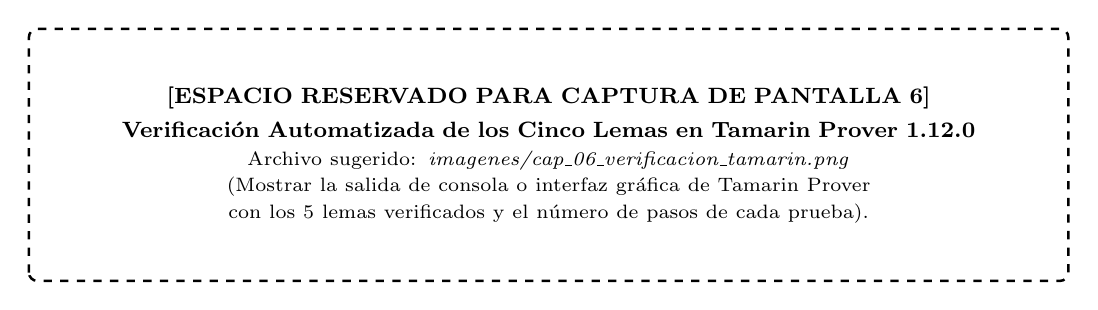
\begin{tikzpicture}
		\draw[line width=0.9pt, dashed, draw=black, fill=white, rounded corners=3pt] (0,0) rectangle (13.2, 3.2);
		\node[align=center, font=\footnotesize\rmfamily, text width=11.8cm] at (6.6, 1.6) {
			\textbf{[ESPACIO RESERVADO PARA CAPTURA DE PANTALLA 6]}\\[3pt]
			\textbf{Verificación Automatizada de los Cinco Lemas en Tamarin Prover 1.12.0}\\[2pt]
			\scriptsize Archivo sugerido: \textit{imagenes/cap\_06\_verificacion\_tamarin.png}\\
			\scriptsize (Mostrar la salida de consola o interfaz gráfica de Tamarin Prover con los 5 lemas verificados y el número de pasos de cada prueba).
		};
	\end{tikzpicture}
	\caption{Verificación formal de lemas en Tamarin Prover.}
	\label{fig:cap_tamarin_prover}
	\par\vspace{2pt}{\footnotesize\textit{Fuente: Elaboración propia.}}
\end{figure}

El lema de \textbf{unicidad} se cumple de forma incondicional gracias al consumo del hecho lineal en el servidor; el \textbf{secreto del voto} se preserva siempre que la clave privada $dk_{\text{AC}}$ de la Autoridad de Conteo no sea filtrada; y los lemas de \textbf{autenticidad} e \textbf{integridad} se sostienen mientras las claves privadas de firma de los electores y de la Autoridad de Registro permanezcan seguras. Como límites declarados del modelo simbólico se dejan registrados la prueba de equivalencia observacional por bi-sistemas (que excede la memoria por explosión de estados), la exclusión de colusión entre servidor y registro (Supuesto S3) y la coacción física presencial fuera del sistema.

\section{Implementación del Protocolo Clásico de Control (Línea Base RSA/ECDSA)}
\label{sec:implementacion_clasica}
% =============================================================================

Para contrastar experimentalmente en el Capítulo 4 el desempeño del protocolo post-cuántico propuesto bajo condiciones idénticas de hardware y arquitectura de software, se implementó un protocolo clásico de referencia que conserva el mismo flujo de validación, las mismas pantallas y la misma estructura de datos, sustituyendo únicamente las primitivas de retículos por los estándares asimétricos tradicionales:

\begin{itemize}
	\item \textbf{Cifrado asimétrico clásico:} Esquema RSA-OAEP con módulo de 2048 bits, exponente público estándar 65537 y función resumen SHA-256 (112 bits de seguridad clásica, vulnerable al algoritmo cuántico de Shor).
	\item \textbf{Firma digital clásica:} Esquema de curvas elípticas ECDSA sobre la curva P-256 del NIST con SHA-256 (128 bits de seguridad clásica, igualmente vulnerable al algoritmo de Shor).
	\item \textbf{Componente simétrico constante:} Se mantiene idéntico el cifrado autenticado AES-256-GCM y el resumen de 256 bits para aislar como única variable independiente el cambio de las primitivas de clave pública.
\end{itemize}

En la Tabla \ref{tab:correspondencia_modulos_didactico} se presenta la equivalencia funcional uno a uno entre los módulos del sistema post-cuántico y los del sistema clásico de control.

\begingroup
\renewcommand{\arraystretch}{1.2}
\setlength{\tabcolsep}{4pt}
\begin{table}[!htbp]
	\centering
	\footnotesize
	\begin{tabular}{|>{\raggedright\arraybackslash}p{3.2cm}|>{\raggedright\arraybackslash}p{5.0cm}|>{\raggedright\arraybackslash}p{5.4cm}|}
		\hline
		\textbf{Componente Lógico} & \textbf{Implementación Post-Cuántica (PQC)} & \textbf{Implementación Clásica de Control} \\
		\hline
		Encapsulamiento / Cifrado & ML-KEM-768 (Estándar FIPS 203) & RSA-OAEP-2048 (Estándar RFC 8017) \\
		\hline
		Esquema de Firma Digital & ML-DSA-65 (Estándar FIPS 204) & ECDSA Curva P-256 (Estándar FIPS 186-4) \\
		\hline
		Núcleo Criptográfico & Implementación propia FIPS 202, 203 y 204 (C/Python) & Módulo clásico sobre OpenSSL (RSA/ECDSA) \\
		\hline
		Entidades del Protocolo & Votante, AR, SV y AC post-cuánticos & Votante, AR, SV y AC clásicos equivalentes \\
		\hline
		Banco de Evaluación & Corredor experimental (300 corridas, lotes de 10 a 1000 votantes) & Corredor experimental bajo idénticas cargas \\
		\hline
		Tamaño Paquete de Voto & \textbf{16293 bytes}* & \textbf{1196 bytes} \\
		\hline
	\end{tabular}
	\caption{Correspondencia entre los módulos post-cuántico y clásico.}
	\label{tab:correspondencia_modulos_didactico}
	\par\vspace{3pt}{\footnotesize\textit{Fuente: Elaboración propia (*medición en formato JSON con campos en hexadecimal y credencial anidada).}}
\end{table}
\endgroup

Esta simetría arquitectónica garantiza que toda variación en los tiempos de ejecución o en el tamaño de los paquetes medida durante las 300 corridas experimentales obedezca exclusivamente al comportamiento algebraico de ML-KEM-768 y ML-DSA-65 frente a RSA-2048 y ECDSA P-256, cuyos resultados estadísticos se analizan en detalle en el Capítulo 4.

